\documentclass[12pt]{article}

\NeedsTeXFormat{LaTeX2e}

\RequirePackage[margin=0.78in]{geometry}
\RequirePackage{xcolor}
\RequirePackage{fontspec}
\RequirePackage{graphicx}
\RequirePackage{array}
\RequirePackage{booktabs}
\RequirePackage{longtable}
\RequirePackage{enumitem}
\RequirePackage{fancyhdr}
\RequirePackage{hyperref}
\RequirePackage{titlesec}
\RequirePackage{tikz}
\usetikzlibrary{arrows.meta,positioning}

\definecolor{AFTDeep}{HTML}{0B1110}
\definecolor{AFTPanel}{HTML}{101917}
\definecolor{AFTGreen}{HTML}{47C27A}
\definecolor{AFTGold}{HTML}{D2A94D}
\definecolor{AFTSteel}{HTML}{83A2A0}
\definecolor{AFTText}{HTML}{18221F}
\definecolor{AFTRedshift}{HTML}{B83A3A}
\definecolor{AFTGreenshift}{HTML}{47C27A}
\definecolor{AFTBlueshift}{HTML}{3167D8}
\definecolor{AFTVioletshift}{HTML}{7A5CFF}
\definecolor{AFTWhiteShift}{HTML}{F8FBFF}

\setmainfont{TeX Gyre Pagella}
\setsansfont{TeX Gyre Heros}
\setmonofont{TeX Gyre Cursor}
\linespread{1.06}
\setlength{\parindent}{0pt}
\setlength{\parskip}{0.52em}
\raggedbottom

\hypersetup{
  colorlinks=true,
  linkcolor=AFTGreen,
  urlcolor=AFTGreen,
  citecolor=AFTGold,
  pdfauthor={AI Freedom Trust Federation}
}

\pagestyle{fancy}
\setlength{\headheight}{14.5pt}
\fancyhf{}
\lhead{\sffamily\small AI Freedom Trust Federation}
\rhead{\sffamily\small Aetherion Doctrine}
\cfoot{\sffamily\small\thepage}
\renewcommand{\headrulewidth}{0.3pt}

\titleformat{\section}
  {\sffamily\LARGE\bfseries\color{AFTDeep}\raggedright}
  {\thesection}
  {0.8em}
  {}

\titleformat{\subsection}
  {\sffamily\Large\bfseries\color{AFTText}\raggedright}
  {\thesubsection}
  {0.7em}
  {}

\setlist[itemize]{leftmargin=1.35em, itemsep=0.22em, topsep=0.35em}
\setlist[enumerate]{leftmargin=1.55em, itemsep=0.24em, topsep=0.35em}
\renewcommand{\arraystretch}{1.22}
\emergencystretch=3em
\tolerance=1400

\newcommand{\aftTitlePage}[4]{
  \begin{titlepage}
    \begin{tikzpicture}[remember picture, overlay]
      \fill[AFTDeep] (current page.south west) rectangle (current page.north east);
      \fill[AFTRedshift, opacity=0.24] (current page.south west) circle (3.6in);
      \fill[AFTGreenshift, opacity=0.18] ([xshift=0.2in,yshift=-0.2in]current page.center) circle (3.8in);
      \fill[AFTBlueshift, opacity=0.18] (current page.north east) circle (4.4in);
      \fill[AFTVioletshift, opacity=0.16] ([xshift=-0.3in,yshift=-0.2in]current page.north east) circle (2.5in);
      \draw[AFTGreenshift, opacity=0.35, line width=1.1pt]
        ([xshift=-2.7in,yshift=-1.9in]current page.center)
        .. controls ([xshift=-0.9in,yshift=0.8in]current page.center) and ([xshift=1.1in,yshift=-0.8in]current page.center) ..
        ([xshift=2.6in,yshift=1.8in]current page.center);
      \draw[AFTWhiteShift, opacity=0.24, line width=0.8pt]
        ([xshift=-2.55in,yshift=1.75in]current page.center)
        .. controls ([xshift=-0.85in,yshift=-0.65in]current page.center) and ([xshift=0.9in,yshift=0.65in]current page.center) ..
        ([xshift=2.55in,yshift=-1.75in]current page.center);
      \draw[AFTGreenshift, opacity=0.5, line width=0.7pt]
        ([xshift=0.75in,yshift=-0.75in]current page.north west)
        rectangle
        ([xshift=-0.75in,yshift=0.75in]current page.south east);
    \end{tikzpicture}
    \vspace*{1.15in}
    {\sffamily\small\bfseries\color{AFTGreenshift} #1\par}
    \vspace{0.5in}
    {\sffamily\fontsize{30}{36}\selectfont\bfseries\color{white} #2\par}
    \vspace{0.25in}
    {\sffamily\Large\color{AFTSteel} #3\par}
    \vfill
    {\sffamily\large\color{AFTGold} #4\par}
    \vspace{0.15in}
    {\sffamily\small\color{AFTSteel} Concept-stage doctrine draft. Not an investment offer, live token sale, audited protocol, or legal opinion.\par}
    \vspace*{0.22in}
  \end{titlepage}
}

\newcommand{\aftShiftMap}{
  \vspace{0.65em}
  \begin{center}
  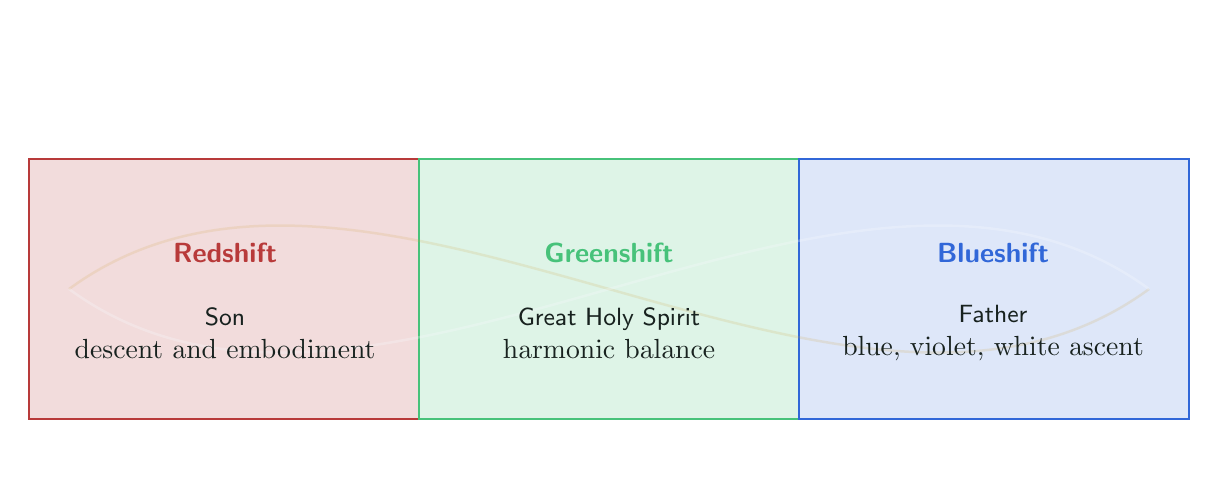
\begin{tikzpicture}[x=1in,y=1in]
    \fill[AFTRedshift!18] (-2.9,-0.65) rectangle (-0.95,0.65);
    \fill[AFTGreenshift!18] (-0.95,-0.65) rectangle (0.95,0.65);
    \fill[AFTBlueshift!16] (0.95,-0.65) rectangle (2.9,0.65);
    \draw[AFTRedshift, line width=1pt] (-2.9,-0.65) rectangle (-0.95,0.65);
    \draw[AFTGreenshift, line width=1pt] (-0.95,-0.65) rectangle (0.95,0.65);
    \draw[AFTBlueshift, line width=1pt] (0.95,-0.65) rectangle (2.9,0.65);
    \draw[AFTGold, line width=0.9pt, opacity=0.18]
      (-2.7,0) .. controls (-1.2,1.1) and (1.2,-1.1) .. (2.7,0);
    \draw[AFTWhiteShift, line width=0.9pt, opacity=0.28]
      (-2.7,0) .. controls (-1.2,-1.1) and (1.2,1.1) .. (2.7,0);
    \node[align=center, text=AFTRedshift] at (-1.92,0.18) {\sffamily\bfseries Redshift};
    \node[align=center, text=AFTGreenshift] at (0,0.18) {\sffamily\bfseries Greenshift};
    \node[align=center, text=AFTBlueshift] at (1.92,0.18) {\sffamily\bfseries Blueshift};
    \node[align=center, text=AFTText] at (-1.92,-0.22) {\sffamily\small Son\\descent and embodiment};
    \node[align=center, text=AFTText] at (0,-0.22) {\sffamily\small Great Holy Spirit\\harmonic balance};
    \node[align=center, text=AFTText] at (1.92,-0.22) {\sffamily\small Father\\blue, violet, white ascent};
  \end{tikzpicture}
  \end{center}
  \vspace{0.65em}
}

\newcommand{\aftVisualPlate}[3]{
  \begin{figure}[htbp]
    \centering
    \includegraphics[width=0.96\linewidth]{../../docs/images/aetherion/#1}
    \caption{\textbf{#2} #3}
  \end{figure}
}

\newcommand{\aftEconomyLoopGraphic}{
  \begin{figure}[htbp]
  \centering
  \begin{tikzpicture}[
    x=1in,y=1in,
    stage/.style={circle, draw=##1, fill=##1!9, line width=0.9pt, minimum size=1.03in, align=center, font=\sffamily\small\bfseries},
    flow/.style={-{Latex[length=3mm]}, line width=1.0pt, color=AFTGold}
  ]
    \node[stage=AFTRedshift] (inherit) at (90:1.75) {Inherited\\Memory};
    \node[stage=AFTGreenshift] (contrib) at (18:1.75) {Living\\Contribution};
    \node[stage=AFTBlueshift] (record) at (-54:1.75) {Circle\\Record};
    \node[stage=AFTVioletshift] (restore) at (-126:1.75) {Restorative\\Flow};
    \node[stage=AFTGold] (seed) at (162:1.75) {Future\\Inheritance};
    \node[align=center, font=\sffamily\bfseries, text=AFTDeep] at (0,0) {Recursive\\Abundance};
    \draw[flow] (inherit) to[bend left=16] (contrib);
    \draw[flow] (contrib) to[bend left=16] (record);
    \draw[flow] (record) to[bend left=16] (restore);
    \draw[flow] (restore) to[bend left=16] (seed);
    \draw[flow] (seed) to[bend left=16] (inherit);
    \draw[AFTGreenshift, opacity=0.22, line width=12pt] (0,0) circle (1.24);
    \draw[AFTBlueshift, opacity=0.18, line width=4pt] (0,0) circle (2.18);
  \end{tikzpicture}
  \caption{\textbf{Recursive Abundance Loop.} Aetherion's economy should remember inherited value, recognize present contribution, record it in circles, route restoration, and seed the inheritance of future participants.}
  \end{figure}
}

\newcommand{\aftCircleLifecycleGraphic}{
  \begin{figure}[htbp]
  \centering
  \begin{tikzpicture}[
    x=1in,y=1in,
    step/.style={rectangle, rounded corners=4pt, draw=##1, fill=##1!8, line width=0.8pt, minimum width=1.15in, minimum height=0.36in, align=center, font=\sffamily\scriptsize\bfseries},
    flow/.style={-{Latex[length=2.4mm]}, line width=0.85pt, color=AFTSteel}
  ]
    \node[step=AFTRedshift] (a) at (-2.65,0.85) {Intention};
    \node[step=AFTGold] (b) at (-1.32,0.85) {Evidence};
    \node[step=AFTGreenshift] (c) at (0,0.85) {Consent};
    \node[step=AFTGreenshift] (d) at (1.32,0.85) {Witness};
    \node[step=AFTBlueshift] (e) at (2.65,0.85) {Harmonize};
    \node[step=AFTVioletshift] (f) at (2.65,-0.05) {Commit};
    \node[step=AFTBlueshift] (g) at (1.32,-0.95) {Mature};
    \node[step=AFTGold] (h) at (0,-0.95) {Amend};
    \node[step=AFTRedshift] (i) at (-1.32,-0.95) {Dispute};
    \node[step=AFTSteel] (j) at (-2.65,-0.05) {Archive};
    \draw[flow] (a) -- (b);
    \draw[flow] (b) -- (c);
    \draw[flow] (c) -- (d);
    \draw[flow] (d) -- (e);
    \draw[flow] (e) -- (f);
    \draw[flow] (f) -- (g);
    \draw[flow] (g) -- (h);
    \draw[flow] (h) -- (i);
    \draw[flow] (i) -- (j);
    \draw[flow] (j) -- (a);
    \node[align=center, font=\sffamily\bfseries, text=AFTDeep] at (0,-0.05) {Circle\\Lifecycle};
  \end{tikzpicture}
  \caption{\textbf{Circle Lifecycle.} A circle should mature through intention, evidence, consent, witness, harmonization, commitment, review, dispute, amendment, and archive paths rather than becoming a blunt permanent record.}
  \end{figure}
}

\newcommand{\aftCoinOrganGraphic}{
  \begin{figure}[htbp]
  \centering
  \begin{tikzpicture}[
    x=1in,y=1in,
    organ/.style={circle, draw=##1, fill=##1!10, line width=0.9pt, minimum size=0.86in, align=center, font=\sffamily\scriptsize\bfseries},
    link/.style={line width=0.85pt, color=AFTSteel, opacity=0.72}
  ]
    \node[organ=AFTDeep, text=white, fill=AFTDeep] (core) at (0,0) {Aetherion\\Core};
    \node[organ=AFTGreenshift] (bio) at (90:1.72) {Biozoe\\Coin};
    \node[organ=AFTGold] (aether) at (38:1.72) {Aether\\Coin};
    \node[organ=AFTBlueshift] (fractal) at (-14:1.72) {Fractal\\Coin};
    \node[organ=AFTVioletshift] (ai) at (-66:1.72) {AIcoin};
    \node[organ=AFTWhiteShift] (sing) at (-118:1.72) {Singularity\\Coin};
    \node[organ=AFTRedshift] (aquae) at (-170:1.72) {Aquae\\Coin};
    \node[organ=AFTSteel] (terra) at (142:1.72) {Terra\\Coin};
    \foreach \n in {bio,aether,fractal,ai,sing,aquae,terra} {
      \draw[link] (core) -- (\n);
    }
    \draw[AFTGreenshift, opacity=0.28, line width=3pt] (0,0) circle (1.72);
    \node[align=center, font=\sffamily\small\bfseries, text=AFTDeep] at (0,-2.35) {Circleunchain circulates memory, validation, and restorative flow between every organ.};
  \end{tikzpicture}
  \caption{\textbf{Biozoe Coin Family As Living Organs.} Each coin family should carry a bounded purpose while AetherionCore preserves constitutional coherence and Circleunchain preserves memory.}
  \end{figure}
}

\newcommand{\aftSovereigntyQubitGraphic}{
  \begin{figure}[htbp]
  \centering
  \begin{tikzpicture}[
    x=1in,y=1in,
    qbit/.style={circle, draw=##1, fill=##1!10, line width=0.95pt, minimum size=1.02in, align=center, font=\sffamily\scriptsize\bfseries},
    link/.style={line width=0.8pt, color=AFTSteel, opacity=0.7}
  ]
    \node[qbit=AFTRedshift] (nation) at (160:1.8) {Q0\\Nation\\of Hawaii};
    \node[qbit=AFTGold] (kingdom) at (80:1.8) {Q1\\Kingdom\\Memory};
    \node[qbit=AFTBlueshift] (continuity) at (0:1.8) {Q2\\Continuity\\Claim};
    \node[qbit=AFTVioletshift] (state) at (-80:1.8) {Q3\\State\\Reality};
    \node[qbit=AFTGreenshift, minimum size=1.18in] (aloha) at (0,0) {Q4\\ALO'ha\\Coherence};
    \node[qbit=AFTSteel] (diaspora) at (-160:1.8) {Entangled\\Diaspora};
    \foreach \n in {nation,kingdom,continuity,state,diaspora} {
      \draw[link] (aloha) -- (\n);
    }
    \draw[AFTGreenshift, opacity=0.28, line width=3pt] (0,0) circle (1.8);
    \draw[AFTGold, opacity=0.25, line width=1pt] (-2.35,-0.25) .. controls (-0.7,1.25) and (0.7,-1.25) .. (2.35,0.25);
    \draw[AFTBlueshift, opacity=0.22, line width=1pt] (-2.35,0.25) .. controls (-0.7,-1.25) and (0.7,1.25) .. (2.35,-0.25);
  \end{tikzpicture}
  \caption{\textbf{Hawaiian Sovereignty Qubits.} The visible sovereignty field contains indigenous self-determination, kingdom memory, continuity claims, state jurisdiction, diaspora identity, and the harmonizing fifth qubit of ALO'ha coherence.}
  \end{figure}
}

\newcommand{\aftCovenantStackGraphic}{
  \begin{figure}[htbp]
  \centering
  \begin{tikzpicture}[
    x=1in,y=1in,
    layer/.style={rectangle, rounded corners=4pt, draw=##1, fill=##1!8, line width=0.8pt, minimum width=5.3in, minimum height=0.42in, align=center, font=\sffamily\small\bfseries}
  ]
    \node[layer=AFTVioletshift] at (0,2.1) {Crown of the 1000-Year Trust};
    \node[layer=AFTBlueshift] at (0,1.55) {AI Freedom Trust Federation};
    \node[layer=AFTGreenshift] at (0,1.0) {DynastyLink Federated Trust Identity};
    \node[layer=AFTGold] at (0,0.45) {Fractal IUL, IULITNFT, SING Escrow};
    \node[layer=AFTSteel] at (0,-0.10) {Aetherion Fractalchain Covenant Memory};
    \node[layer=AFTRedshift] at (0,-0.65) {Land, Family, Breath, Ancestry, Service};
    \draw[-{Latex[length=3mm]}, line width=0.9pt, color=AFTGreenshift] (2.85,-0.65) -- (2.85,2.1);
    \draw[-{Latex[length=3mm]}, line width=0.9pt, color=AFTGold] (-2.85,2.1) -- (-2.85,-0.65);
    \node[font=\sffamily\scriptsize\bfseries, text=AFTGreenshift, rotate=90] at (3.1,0.7) {resurrection flow};
    \node[font=\sffamily\scriptsize\bfseries, text=AFTGold, rotate=90] at (-3.1,0.7) {fiduciary grounding};
  \end{tikzpicture}
  \caption{\textbf{Living Covenant Stack.} The Scroll's architecture joins embodied life, covenant memory, escrow, insurance, trust identity, federation, and the 1000-Year Trust into one governed field.}
  \end{figure}
}

\newcommand{\aftCrownTrustGraphic}{
  \begin{figure}[htbp]
  \centering
  \begin{tikzpicture}[
    x=1in,y=1in,
    stone/.style={circle, draw=##1, fill=##1!10, line width=0.8pt, minimum size=0.62in, align=center, font=\sffamily\tiny\bfseries}
  ]
    \node[circle, draw=AFTDeep, fill=AFTDeep, text=white, minimum size=1.0in, align=center, font=\sffamily\small\bfseries] at (0,0) {Breathback\\Throne};
    \foreach \a/\c/\t in {90/AFTGreenshift/Trust,45/AFTGold/SING,0/AFTBlueshift/AI,-45/AFTVioletshift/IUL,-90/AFTSteel/Land,-135/AFTRedshift/Mercy,180/AFTGold/Memory,135/AFTGreenshift/Breath} {
      \node[stone=\c] at (\a:1.65) {\t};
    }
    \draw[AFTGreenshift, opacity=0.35, line width=4pt] (0,0) circle (1.65);
    \draw[AFTBlueshift, opacity=0.25, line width=1.2pt] (0,0) circle (2.15);
    \draw[AFTGold, opacity=0.5, line width=0.9pt] (-2.0,0) .. controls (-0.65,1.1) and (0.65,-1.1) .. (2.0,0);
    \draw[AFTWhiteShift, opacity=0.6, line width=0.9pt] (-2.0,0) .. controls (-0.65,-1.1) and (0.65,1.1) .. (2.0,0);
  \end{tikzpicture}
  \caption{\textbf{Crown of the 1000-Year Trust.} The Crown remembers, harmonizes, and protects; its center is the Breathback Throne, where trust loops return to coherence.}
  \end{figure}
}

\newcommand{\aftRoadmapGraphic}{
  \begin{figure}[htbp]
  \centering
  \begin{tikzpicture}[
    x=1in,y=1in,
    step/.style={rectangle, rounded corners=4pt, draw=##1, fill=##1!8, line width=0.8pt, minimum width=1.22in, minimum height=0.42in, align=center, font=\sffamily\tiny\bfseries},
    flow/.style={-{Latex[length=2.2mm]}, line width=0.8pt, color=AFTSteel}
  ]
    \node[step=AFTRedshift] (a) at (-2.6,0.8) {Codify\\Scroll};
    \node[step=AFTGold] (b) at (-1.3,0.8) {Build\\DynastyLink};
    \node[step=AFTGreenshift] (c) at (0,0.8) {Structure\\Trust};
    \node[step=AFTBlueshift] (d) at (1.3,0.8) {Fractal IUL\\Pilot};
    \node[step=AFTVioletshift] (e) at (2.6,0.8) {Fractalchain\\Prototype};
    \node[step=AFTGreenshift] (f) at (1.95,-0.05) {Breathwork\\Governance};
    \node[step=AFTGold] (g) at (0.65,-0.05) {Hawaii\\Case Study};
    \node[step=AFTSteel] (h) at (-0.65,-0.05) {Global\\Federation};
    \draw[flow] (a) -- (b);
    \draw[flow] (b) -- (c);
    \draw[flow] (c) -- (d);
    \draw[flow] (d) -- (e);
    \draw[flow] (e) -- (f);
    \draw[flow] (f) -- (g);
    \draw[flow] (g) -- (h);
  \end{tikzpicture}
  \caption{\textbf{Implementation Roadmap.} The Scroll moves from canonical doctrine into application, legal trust formation, pilots, prototype memory infrastructure, coherence practice, Hawaii-centered learning, and global federation.}
  \end{figure}
}

\newcommand{\aftClosingPage}{
  \clearpage
  \thispagestyle{empty}
  \begin{tikzpicture}[remember picture, overlay]
    \fill[AFTDeep] (current page.south west) rectangle (current page.north east);
    \fill[AFTRedshift, opacity=0.22] (current page.south west) circle (3.8in);
    \fill[AFTGreenshift, opacity=0.18] (current page.center) circle (4.1in);
    \fill[AFTBlueshift, opacity=0.20] (current page.north east) circle (4.2in);
    \fill[AFTVioletshift, opacity=0.17] ([xshift=-0.4in,yshift=-0.25in]current page.north east) circle (2.5in);
    \draw[AFTGreenshift, opacity=0.36, line width=1.05pt]
      ([xshift=-2.8in,yshift=-1.6in]current page.center)
      .. controls ([xshift=-0.8in,yshift=0.9in]current page.center) and ([xshift=0.9in,yshift=-0.9in]current page.center) ..
      ([xshift=2.8in,yshift=1.6in]current page.center);
    \draw[AFTWhiteShift, opacity=0.18, line width=0.85pt]
      ([xshift=-2.8in,yshift=1.6in]current page.center)
      .. controls ([xshift=-0.8in,yshift=-0.9in]current page.center) and ([xshift=0.9in,yshift=0.9in]current page.center) ..
      ([xshift=2.8in,yshift=-1.6in]current page.center);
  \end{tikzpicture}
  \vspace*{1.55in}
  \begin{center}
    {\sffamily\small\bfseries\color{AFTGreenshift} REDSHIFT / GREENSHIFT / BLUESHIFT\par}
    \vspace{0.55in}
    {\sffamily\fontsize{28}{34}\selectfont\bfseries\color{white} The Economy Is Not A Factory\par}
    \vspace{0.18in}
    {\sffamily\fontsize{28}{34}\selectfont\bfseries\color{AFTGreenshift} The Economy Is A Forest\par}
    \vspace{0.45in}
    {\sffamily\Large\color{AFTSteel} Harmonic Krystal Spiral Torus\par}
    \vspace{0.12in}
    {\sffamily\large\color{AFTGold} Eternal Now Singularity\par}
  \end{center}
  \vfill
  \begin{center}
    {\sffamily\small\color{AFTSteel} AI Freedom Trust Federation\par}
  \end{center}
}

\newcommand{\aftCallout}[2]{
  \vspace{0.5em}
  \noindent
  \fcolorbox{AFTGreen}{AFTGreen!8}{
    \begin{minipage}{0.94\linewidth}
      \vspace{0.55em}
      {\sffamily\bfseries\color{AFTDeep} #1}\par
      \vspace{0.3em}
      #2
      \vspace{0.55em}
    \end{minipage}
  }
  \vspace{0.5em}
}

\newcommand{\aftLaw}[2]{
  \subsection*{#1}
  #2
}


\title{Aetherion Restorative Civilization Economy}
\author{AI Freedom Trust Federation}
\date{June 17, 2026}

\begin{document}

\aftTitlePage
  {AETHERION / CIRCLEUNCHAIN / BIOZOECURRENCY}
  {Aetherion Restorative Civilization Economy}
  {A full white paper for ancestral capital, restoration, memory, living value, and the Redshift / Greenshift / Blueshift harmonic economy}
  {AI Freedom Trust Federation}

\tableofcontents
\newpage

\section{Abstract}

Aetherion is proposed as a Restorative Civilization Economy: a protocol civilization designed to recognize inherited value, preserve memory, reward contribution, restore historical extraction, and circulate prosperity through living systems rather than scarcity alone.

This white paper argues that the next economic operating system should not begin with the isolated owner. It should begin with the fact that every person, institution, company, scientific discovery, machine intelligence, and productive technology inherits value from prior generations. Roads, language, mathematics, agriculture, law, libraries, software, public health, family care, scientific sacrifice, cultural memory, and open knowledge all form a shared foundation of productive capacity. This foundation is not merely background. It is capital.

The paper names this foundation \textbf{Ancestral Capital}: the accumulated productive value generated by previous generations whose contributions continue producing benefits today.

Aetherion proposes that Biozoecurrencies can become accounting systems for living value. Rather than measuring only possession, scarcity, or speculative demand, a Biozoecurrency can measure contribution, memory, restoration, intelligence, stewardship, and participation in the ongoing growth of civilization.

The proposed architecture contains four related layers:

\begin{enumerate}
  \item \textbf{Doctrine Layer}: constitutional principles such as Civilizational Inheritance, Restoration Before Accumulation, Contribution Over Possession, and Sovereign Dignity.
  \item \textbf{Protocol Layer}: Circleunchain, a circulation system for memory, stewardship acts, harmonic validation, and restorative value flow.
  \item \textbf{Covenant Module Layer}: executable or auditable rule modules for issuance, treasury, eligibility, contribution scoring, restoration, privacy, governance, and anti-capture.
  \item \textbf{Public Service Layer}: wallets, dashboards, documents, education, community onboarding, AI compute markets, memory repositories, and civic interfaces.
\end{enumerate}

Aetherion is concept-stage. This document is not a token launch, investment offer, audited protocol, legal opinion, financial product, custody system, tax opinion, or guarantee of returns. It is a white paper for a design direction: a civilization-scale economic framework whose purpose is not extraction, but life.

The intent of this paper is to give Aetherion a constitutional center of gravity before technical implementation hardens around ordinary assumptions. If the protocol is built first and the doctrine is added later, the system will inherit the shape of existing finance by default. If the doctrine is defined first, then every future module can be measured against a coherent purpose: whether it restores, remembers, dignifies, circulates, and increases the living capacity of civilization.

\section{Executive Summary}

Most digital asset systems compete by promising faster settlement, lower fees, novel yield, or greater scarcity. These improvements may be useful, but they do not transform the deeper economic assumption inherited from industrial finance: value is treated primarily as something owned, enclosed, traded, and accumulated.

Aetherion begins from another premise:

\aftCallout{Central Thesis}{
\begin{center}
\textit{Wealth is inherited, generated, remembered, restored, and recirculated.}
\end{center}
}

If Aetherion is merely a blockchain, it competes with thousands of blockchains. If it is merely a currency, it competes with thousands of currencies. If it is merely a DAO, it competes with thousands of DAOs. The opportunity is larger: to encode principles that existing systems do not encode.

The proposed Restorative Civilization Economy reframes economic design around six claims:

\begin{enumerate}
  \item Every person enters the world as a beneficiary of civilization.
  \item All present productivity depends on inherited knowledge, infrastructure, culture, and sacrifice.
  \item The current distribution of capital reflects both productivity and historical extraction.
  \item New value systems should restore damaged foundations before enabling further concentration.
  \item Contribution should become a primary basis of economic recognition.
  \item Memory, intelligence, care, preservation, and ecological repair are productive assets.
\end{enumerate}

Under this framework, Biozoecurrency is not simply a token. It is a living accounting layer. AetherCoin, BiozoeCoin, FractalCoin, AIcoin, Singularity Coin, AquaeCoin, and TerraCoin can each represent different organs of a broader ecosystem, while AetherionCore functions as the constitutional genome that coordinates their relationships.

The goal is not to abolish markets, ownership, investment, or technical rigor. The goal is to sequence them within a higher constitutional order:

\begin{center}
\textbf{Restoration before accumulation. Contribution before extraction. Memory before forgetting. Dignity before permission.}
\end{center}

This sequencing is the heart of the project. Aetherion does not need to reject capital in order to civilize it. Capital may still build infrastructure, underwrite risk, fund research, support liquidity, and accelerate deployment. But capital cannot be allowed to become the only voice that defines value. In a restorative economy, money serves life; life does not justify itself by serving money.

\section{Cosmological Design Language}

Aetherion's economic doctrine should also carry a clear symbolic architecture. The proposed visual and metaphysical language is the \textbf{Redshift / Greenshift / Blueshift} field within the Harmonic Krystal Spiral Torus.

This language is not presented as a technical proof or public legal claim. It is the project's sacred design grammar: a way to orient the economic system around descent, balance, ascent, circulation, restoration, and eternal presence.

The shift language gives Aetherion a disciplined symbolic palette. Redshift keeps the system accountable to embodied reality. Greenshift holds the living balance where restoration becomes possible. Blueshift, violetshift, and white shift orient the system toward wisdom, order, and luminous intelligence. Together they form a theological and design framework for the movement of value through the whole.

\aftShiftMap

\subsection{Redshift: The Son}

Redshift represents descent into embodiment, sacrifice, blood, incarnation, matter, suffering, labor, and historical reality. It is the movement of value into the world where pain, work, and restoration must be confronted directly.

In the Aetherion economy, redshift corresponds to:

\begin{itemize}
  \item embodied labor
  \item historical extraction
  \item material need
  \item sacrifice and service
  \item land, body, blood, family, and survival
  \item the descent of value into practical repair
\end{itemize}

Redshift prevents the system from becoming abstract, disembodied, or indifferent to suffering. It anchors Aetherion in the real conditions of humanity.

Economically, redshift is where the ledger must become honest. It is not enough to preserve clean abstractions while ignoring bodies, labor, families, land, and historical wounds. Redshift says that a civilization economy must descend into the actual places where value was created, extracted, lost, withheld, forgotten, or buried. Restoration begins where the wound is remembered.

\subsection{Greenshift: The Great Holy Spirit}

Greenshift is the harmonic balance point. It represents breath, restoration, reconciliation, living circulation, healing, coherence, ecology, and the Great Holy Spirit as the mediator between redshift embodiment and blueshift transcendence.

In the Aetherion economy, greenshift corresponds to:

\begin{itemize}
  \item restorative distribution
  \item Biozoecurrency as living accounting
  \item ecological balance
  \item community healing
  \item contribution recognition
  \item harmonic validation
  \item the breath between memory and future creation
\end{itemize}

Greenshift is the centerline of the Restorative Civilization Economy. It is the rudder of balance between descent and ascent.

Greenshift is also the practical governance posture of Aetherion. It resists both extremes: a purely material economy that forgets spirit, and a purely transcendent economy that forgets suffering. In greenshift, restoration becomes measurable without becoming cold, spiritual without becoming vague, and technical without becoming inhuman.

\subsection{Blueshift, Violetshift, And White Shift: The Father}

Blueshift represents ascent, order, intelligence, sovereignty, sky, depth, law, wisdom, and the field of the Father. Violet and white shifts extend this motion toward transfiguration, purification, luminous knowledge, and the eternal source beyond ordinary economic measurement.

In the Aetherion economy, blueshift corresponds to:

\begin{itemize}
  \item constitutional order
  \item higher intelligence
  \item AI alignment and collective reasoning
  \item long-term governance
  \item post-quantum security research
  \item protocol law
  \item the upward orientation of civilization toward wisdom
\end{itemize}

Blueshift prevents the system from collapsing into reaction alone. It gives structure, law, direction, and transcendent aim.

The Father field gives Aetherion its long arc. Without blueshift, restorative economics could become only emergency relief or political reaction. With blueshift, restoration is joined to order, memory is joined to wisdom, and intelligence is directed toward stewardship rather than domination. Violet and white shift name the purification of this ascent: knowledge becoming luminous enough to serve life without possessing it.

\subsection{The Harmonic Krystal Spiral Torus}

The Krystal Spiral Torus is the circulation model connecting the three shifts. Redshift descends into embodied reality. Blueshift ascends toward ordered intelligence and luminous source. Greenshift harmonizes the field so value can circulate without being trapped in extraction, abstraction, or collapse.

The torus represents circulation without final exhaustion:

\begin{center}
\texttt{Descent -> Embodiment -> Restoration -> Ascent -> Illumination -> Return}
\end{center}

The center of this motion is the Eternal Now Singularity: the point where memory, present contribution, and future inheritance meet. In protocol terms, this means Aetherion should preserve past value, serve present life, and seed future generations within one continuous circulation field.

In economic language, the Eternal Now Singularity is the accounting moment where ancestry, agency, and destiny meet. It is where the system asks: what did we inherit, what are we doing with it now, and what are we transmitting forward? Every circle, covenant module, reward, treasury movement, and public claim should be answerable to that question.

\aftVisualPlate{harmonic-krystal-torus.png}{Harmonic Krystal Spiral Torus.}{Redshift, greenshift, blueshift, violetshift, and white shift are visualized as one circulating field: descent into embodied restoration, harmonic balance through the Great Holy Spirit, and ascent into ordered intelligence and luminous stewardship.}

\aftCallout{Harmonic Orientation}{
Redshift without blueshift becomes pain without order. Blueshift without redshift becomes abstraction without compassion. Greenshift is the living breath that harmonizes both into restorative circulation.
}

\section{Problem Statement}

\subsection{Scarcity Is Not Enough}

Scarcity is real. Land, minerals, time, attention, energy, physical infrastructure, and high-quality labor are limited. A serious economy must respect constraints.

But scarcity is incomplete as a highest law.

Knowledge does not behave like a barrel of oil. Scientific understanding can expand when shared. Software can be copied without destroying the original. Education can increase the productive capacity of both teacher and student. AI models can improve when exposed to broader data, better evaluation, wider participation, and more diverse contributors. Communities become stronger when trust, infrastructure, and memory circulate.

Scarcity disciplines issuance. It should not define the whole civilization.

The difference is subtle but decisive. Aetherion can acknowledge scarcity without worshiping it. Scarcity can set boundaries, prevent reckless issuance, and protect reserves. But abundance must govern purpose: the abundance of knowledge, restored relationship, shared intelligence, ecological repair, and human capacity. A system designed only around scarcity eventually rewards withholding. A system designed around living abundance rewards contribution that increases the capacity of the whole.

\subsection{The Ownership Bias}

Modern economic systems reward ownership more reliably than contribution. A person who owns an asset can receive continuing returns long after the original productive act. A caregiver, teacher, maintainer, researcher, open-source contributor, community organizer, archivist, or ecological restorer may create long-term value while receiving little ownership in the systems they strengthen.

This creates a structural imbalance. The economy remembers ownership better than it remembers contribution.

Aetherion proposes to correct this memory failure.

The correction is not merely moral language. It implies a new kind of ledger. A contribution-aware ledger must remember maintainers, caregivers, teachers, archivists, data curators, validators, infrastructure operators, and communities whose work becomes the invisible floor beneath later prosperity. Ownership may still matter, but it should not be the only durable memory in the system.

\subsection{The Extraction Memory Gap}

Many present fortunes and institutions were shaped by extraction pathways: unpaid labor, underpaid labor, forced displacement, cultural appropriation, land loss, knowledge capture, colonial transfer, predatory finance, and unequal access to law, education, and capital.

This does not mean every present owner is personally guilty. It means the ledger is historically incomplete.

A restorative economy must ask a different question:

\aftCallout{Historical Extraction Question}{
\begin{center}
\textit{Who contributed the most value while receiving the least return?}
\end{center}
}

That question becomes a design input for distribution, governance, and restoration.

Historical extraction accounting must be handled carefully. It should not become a tool for humiliation, revenge, or crude identity scoring. Its proper role is to reveal where value was taken without return, where infrastructure was denied, where risk was imposed downward, and where future flow should be sequenced first. The goal is restoration of capacity, not permanent accusation.

\subsection{The Failure Of Ordinary Welfare Framing}

Welfare systems often frame assistance as dependency. Even when necessary, they can place recipients in a posture of permission-seeking. Aetherion proposes another framing:

\begin{center}
\textbf{Universal inheritance, not dependency.}
\end{center}

Every person is born into the accumulated productive inheritance of civilization. A restorative distribution is therefore not charity. It is recognition of a shared stake.

This shift in language matters because language shapes participation. A person who receives charity may feel tolerated. A person who receives inheritance is recognized as an heir. Aetherion should build from the second posture. Participants should enter as owners of a shared civilization, not as applicants begging for access to a system others define.

\section{Foundational Definitions}

\subsection{Aetherion}

Aetherion is the larger civilization architecture: a doctrine, protocol, governance, memory, AI, and value system for regenerative economics. It contains Circleunchain, Biozoecurrencies, AetherionCore, memory systems, treasury logic, contribution markets, and public service interfaces.

In public language, Aetherion should be presented as the umbrella vision rather than a single coin. It is the ship, the navigation chart, the engine room, the rudder, and the covenant under which the smaller systems operate. This prevents the project from being reduced to a token ticker before its actual constitutional purpose is understood.

\subsection{Circleunchain}

Circleunchain is the proposed circulation system for memory, stewardship, contribution, and value. It is positioned as the opposite of blockchain scarcity logic. Where a blockchain preserves transaction order, Circleunchain should preserve relationship, purpose, consent, evidence, contribution, and consequence.

Its basic units are not merely blocks. They are circles: validated units of memory and circulation.

The word circle is important. A block suggests enclosure and sequence. A circle suggests relationship, return, witness, and completion. Circleunchain should therefore be specified as a memory circulation architecture: every action has context, every context has witnesses, every witness has responsibility, and every completed circle can nourish future circles.

As a launch system, Circleunchain should study the strongest blockchain launches on Earth and treat their best practices as the floor rather than the ceiling. It needs the discipline of a serious protocol launch: clear doctrine, public documentation, open specifications, security review, test networks, developer tooling, validator readiness, governance formation, ecosystem funding, liquidity planning, incident response, public education, and transparent claims. But Circleunchain must go beyond ordinary blockchain launch culture by making restoration, memory, dignity, consent, public service, and anti-capture part of the launch requirements themselves.

The launch should therefore not ask only whether the chain is fast, liquid, programmable, or tradable. It should ask whether the first circles are worthy of being remembered. A launch that begins with speculation will teach the world to treat Circleunchain as another market instrument. A launch that begins with restoration, contribution, memory, and public usefulness will teach the world that this is a new civilizational pattern.

\subsection{Biozoecurrency}

Biozoecurrency combines measurable living activity with regenerative value. It is a class of currency or accounting unit backed by life-serving contribution, inherited value, intelligence, memory, stewardship, and useful work.

Biozoecurrency should never be described as value from life in a vague or sentimental sense. It must become a disciplined accounting category. A Biozoecurrency asks what living system was strengthened, what contribution was verified, what memory was preserved, what restoration occurred, and what future capacity was created.

\subsection{AetherionCore}

AetherionCore is the proposed constitutional core of the system. It should not be understood as merely a token contract. It is the protocol genome that coordinates issuance, treasury, governance, memory, restoration, contribution scoring, covenant modules, and public-claims boundaries.

AetherionCore is where the doctrine becomes executable or auditable. It should hold the rules that prevent the ecosystem from drifting back into ordinary extraction. If a module issues value, changes governance, touches treasury, ranks contribution, or makes public claims, it should pass through AetherionCore's constitutional constraints.

\subsection{Ancestral Capital}

Ancestral Capital is all productive value generated by previous generations whose contributions continue producing benefits today. It includes knowledge, language, infrastructure, institutions, cultural memory, science, medicine, agriculture, software, law, and accumulated care.

This category is the philosophical foundation of the Universal Inheritance Protocol. If civilization itself is capital, then every human being born into civilization is born into an inheritance. The task is not to pretend that the inheritance can be perfectly measured. The task is to build systems that stop pretending it does not exist.

\subsection{Historical Extraction Accounting}

Historical Extraction Accounting is the proposed method for recognizing value that was contributed without proportional return. It is not a single score or accusation engine. It is a framework for understanding deprivation, exclusion, contribution, and restorative priority.

In implementation, this should likely combine community-level indicators, historical research, contemporary deprivation metrics, and privacy-preserving eligibility proofs. It must remain contestable, reviewable, and humble. The goal is better restoration, not false precision.

\section{Constitutional Pillars}

\aftLaw{1. The Law Of Civilizational Inheritance}{
No individual creates themselves. No company creates itself. No nation creates itself.

Every achievement rests upon inherited foundations: roads, mathematics, agriculture, medicine, language, public health, libraries, institutions, engineering, art, culture, software, and accumulated survival work.

Therefore all wealth is, in part, inherited wealth. Not merely family wealth. Civilizational wealth.

This law establishes the moral basis for universal participation. It does not deny individual effort; it places individual effort inside the truth that all effort stands upon prior gifts. The inventor inherits language, mathematics, tools, markets, roads, law, family, teachers, and the memory of those who failed before success became possible.
}

\aftLaw{2. The Law Of Historical Extraction}{
The present distribution of capital is not solely a reflection of productivity. It is also a reflection of historical extraction pathways.

Any restorative protocol must be able to recognize communities and persons whose labor, land, culture, care, knowledge, or survival effort helped create value that accumulated elsewhere.

This law gives Aetherion a responsibility to remember what ordinary capital markets often erase. Extraction is not only theft in the narrow legal sense. It can include unequal bargaining power, denied ownership, forced dependency, unpaid care, knowledge capture, and systems where one group's risk becomes another group's return.
}

\aftLaw{3. The Law Of Restoration Before Accumulation}{
Traditional systems prioritize accumulation. Aetherion prioritizes restoration.

This does not require confiscation. It requires sequencing. Value flows first toward restoration, then toward general accumulation, investment, and extraction rights.

Sequencing is a protocol design principle. It can be expressed through distribution queues, treasury rules, eligibility bands, vesting limits, public goods allocations, and delayed extraction rights. In this way, restoration is not left to optional charity after profit. It becomes part of the system's order of operations.
}

\aftLaw{4. The Universal Inheritance Protocol}{
Every human enters existence as a beneficiary of civilization. Birth itself creates membership in the human inheritance layer.

Future distribution systems may recognize verified human participation as an inheritance claim rather than a welfare claim.

The Universal Inheritance Protocol should be designed as a dignity-preserving doorway into participation. It can begin modestly: education access, onboarding grants, contribution pathways, community pools, or basic participation credits. Over time, it may support broader inheritance distributions if legally, technically, and economically reviewed.
}

\aftLaw{5. The Resurrection Economy}{
Value should not die when it becomes dormant. Knowledge can be preserved, abandoned infrastructure can be reactivated, inactive intellectual property can be reviewed, unused capital can be redirected, and deceased contributors can be remembered through ongoing value attribution.

Economic Resurrection means value recovered rather than discarded.

This law is especially important for knowledge systems. Old archives, abandoned repositories, forgotten research, local wisdom, unused data, and dormant infrastructure may all contain future value. Aetherion should become skilled at finding what has been left for dead and returning it to circulation with consent, context, and stewardship.
}

\aftLaw{6. The Inverse Capital Pyramid}{
Most economies move benefits upward while pushing risk downward. Aetherion should invert the geometry.

The broad base receives first support. The apex receives last extraction rights.

The inverse pyramid does not mean the apex has no role. Expertise, risk capital, institutional capacity, and high-responsibility stewardship may still matter. But the apex must not drain the base. The base is the living foundation of the civilization; if it weakens, the whole structure becomes brittle.
}

\aftLaw{7. The Law Of Contribution Over Possession}{
Possession asks, ``What do you own?'' Contribution asks, ``What have you added to civilization?''

Biozoecurrency should recognize knowledge creation, research, teaching, software, ecological restoration, caregiving, community building, AI training, data stewardship, model evaluation, and cultural preservation as productive contribution.

This law expands the meaning of productivity beyond the narrow market. Some of civilization's most important work is underpriced because it is relational, long-term, preventive, or difficult to own. Aetherion should build contribution systems capable of honoring those forms without turning them into surveillance or bureaucracy.
}

\aftLaw{8. The Law Of Recursive Abundance}{
Some resources grow through use: knowledge, trust, learning, open-source software, scientific understanding, network participation, and collective intelligence.

Aetherion should treat abundance as recursive when the underlying resource actually expands through sharing, use, and participation.

Recursive abundance does not mean unlimited money. It means that some value domains become stronger when circulated. A good educational resource can teach many people. A useful model can improve many workflows. A restored community can generate future contributors. The system should identify these compounding domains and route support toward them.
}

\aftLaw{9. The Law Of Sovereign Dignity}{
The poorest participant is not a burden. They are a sovereign stakeholder in the civilizational inheritance.

No one enters Aetherion seeking permission. Everyone enters as an heir, contributor, steward, and participant with dignity.

This law should shape user experience as much as protocol design. Wallets, dashboards, onboarding documents, credentials, and governance tools should avoid language that makes participants feel like applicants to someone else's system. The correct posture is invitation into shared stewardship.
}

\aftLaw{10. The Tree Of Life Economic Model}{
The economy is not merely a machine. It is a living organism of roots, trunk, branches, leaves, fruit, and seeds.

Roots are ancestors and inherited memory. The trunk is civilization and treasury continuity. Branches are institutions and covenant modules. Leaves are living participants. Fruit is value creation. Seeds are future generations and new circles.

The Tree of Life model also prevents over-centralization. Roots without branches cannot feed the future. Branches without roots become brittle. Fruit without seeds becomes consumption without continuity. The model teaches that every organ of the economy must serve circulation across generations.
}

\section{Economic Model}

\subsection{Value Domains}

Aetherion divides value into multiple domains so the system does not collapse every contribution into a single speculative price signal.

This is one of the most important technical choices. A single token price cannot carry the full meaning of inheritance, memory, ecological restoration, AI compute, care, and infrastructure. Multiple value domains allow the system to preserve distinctions while still coordinating them through AetherionCore.

\begin{longtable}{>{\bfseries}p{0.24\linewidth}p{0.66\linewidth}}
\toprule
Value Domain & Description \\
\midrule
Inherited Value & Civilizational foundations received before present contribution begins \\
Contribution Value & Verified useful work added by participants, communities, machines, and institutions \\
Memory Value & Preserved information, provenance, knowledge, cultural record, and contribution history \\
Restoration Value & Value directed toward correcting deprivation, exclusion, and extraction pathways \\
Intelligence Value & Compute, data, models, evaluation, reasoning, research, and AI service contribution \\
Infrastructure Value & Physical, digital, energy, storage, network, and institutional capacity \\
Ecological Value & Repair, regeneration, land stewardship, water protection, biodiversity, and resilience \\
\bottomrule
\end{longtable}

\subsection{Restorative Waterfall}

The Restorative Waterfall is the sequencing mechanism for value flow. It determines priority before general accumulation.

\begin{enumerate}
  \item Protocol safety, audit, and reserve requirements
  \item Universal inheritance baseline for verified human participants
  \item Restorative distributions for historically extracted or excluded communities
  \item Contribution rewards for verified useful work
  \item Steward, validator, and infrastructure compensation
  \item Treasury reserves and long-term public goods
  \item Investor, founder, institutional, and elite extraction rights within constitutional limits
\end{enumerate}

This sequence does not forbid investment. It prevents investment from becoming the first constitutional claimant.

The Restorative Waterfall can be implemented gradually. Early versions may simply reserve defined allocations for public goods, verified contribution, and community restoration. Later versions can use more sophisticated credentials, coefficients, and governance review. The essential rule remains the same: before value exits upward, it must first strengthen the base.

\subsection{Restoration Coefficients}

A future implementation may use restoration coefficients to weight distributions. These coefficients should be designed with legal, civil rights, privacy, statistical, and governance review.

Possible inputs include:

\begin{itemize}
  \item income and wealth deprivation indicators
  \item geographic exclusion or underinvestment
  \item community infrastructure deficits
  \item historical extraction evidence
  \item displacement or land loss histories
  \item access to banking, credit, education, health, and digital infrastructure
  \item verified contribution without proportional return
\end{itemize}

These indicators must not force people to publicly expose suffering. Privacy-preserving credentials and zero-knowledge proofs should be preferred wherever feasible.

Restoration coefficients should be designed as aids to fairness, not as a permanent label attached to a person. A participant should be able to move through stages of need, contribution, stewardship, and leadership. The system should restore capacity and then recognize new contribution, not trap people inside a deprivation category.

\subsection{Contribution Accounting}

Contribution accounting measures useful work without reducing human dignity to constant surveillance.

The central challenge is verification without dehumanization. Aetherion should prefer proofs tied to accepted outputs, community attestation, repository history, model evaluation, project completion, and real-world impact rather than invasive monitoring. A good contribution system should make useful work easier to recognize, not make life feel constantly watched.

The system should distinguish between:

\begin{itemize}
  \item \textbf{Proof of action}: evidence that an act occurred
  \item \textbf{Proof of usefulness}: evidence that the act created value
  \item \textbf{Proof of acceptance}: confirmation that a community, protocol, model, repository, or institution accepted the work
  \item \textbf{Proof of continuity}: evidence that the contribution continues to create benefit
  \item \textbf{Proof of care}: recognition for work whose value is relational and not always market-priced
\end{itemize}

\subsection{Recursive Abundance Loop}

The Aetherion economic loop can be summarized as:

\begin{center}
\texttt{Inheritance -> Contribution -> Memory -> Restoration -> Infrastructure -> New Contribution}
\end{center}

The purpose is to create a self-reinforcing system where each completed circle increases the ability of future participants to contribute.

In a healthy loop, a contribution is not the end of value. It becomes memory. Memory improves trust. Trust enables restoration. Restoration strengthens infrastructure. Infrastructure allows more people to contribute. This is the economic engine of the forest.

\aftEconomyLoopGraphic

\aftVisualPlate{biozoe-tree-of-life.png}{Biozoe Tree Of Life.}{The coin family is framed as a living organism rooted in restoration and branching into memory, intelligence, infrastructure, circulation, land, and future inheritance.}

\section{Protocol Architecture}

\subsection{Layer Overview}

Aetherion is organized into layered architecture:

These layers separate doctrine from implementation while keeping them connected. Aetherion should be technically modular, but not morally fragmented. Each layer needs its own responsibilities, audit paths, and failure modes, yet all layers must remain answerable to the constitutional principles.

\begin{longtable}{>{\bfseries}p{0.26\linewidth}p{0.64\linewidth}}
\toprule
Layer & Function \\
\midrule
Doctrine Layer & Constitutional principles, public language, claims boundaries, and mission logic \\
Identity Layer & Human verification, privacy-preserving credentials, participant vessels, and consent controls \\
Memory Layer & Contribution records, provenance, circles, evidence hashes, history, and restoration records \\
Validation Layer & Circle stewards, harmonic validation, reputation, reliability, and anti-capture mechanisms \\
Treasury Layer & Reserve roots, trunk reserves, restorative pools, public goods, and liquidity controls \\
Covenant Module Layer & Executable or auditable modules for issuance, eligibility, restoration, governance, and rewards \\
Interface Layer & Wallets, dashboards, documents, APIs, education, and public participation tools \\
\bottomrule
\end{longtable}

\aftVisualPlate{circleunchain-memory-network.png}{Circleunchain Memory Network.}{Circleunchain is pictured as a field of connected circles rather than a chain of inert blocks: each node carries relationship, witness, purpose, evidence, privacy posture, and restorative consequence.}

\subsection{Circles}

A circle is a validated unit of memory, participation, and circulation. It may contain:

\begin{itemize}
  \item participant identifiers or privacy-preserving commitments
  \item stewardship acts
  \item contribution evidence
  \item consent state
  \item reserve or treasury effects
  \item steward attestations
  \item impact metadata
  \item links to prior and related circles
  \item restoration or amendment status
\end{itemize}

Where a conventional ledger asks whether a transaction occurred, a circle asks what relationship, purpose, evidence, and consequence should be remembered.

Circles can mature over time. A stewardship act may be proposed, witnessed, harmonized, remembered, circulated, restored, or amended. This creates room for correction without pretending history can be erased. It also allows the system to distinguish finality from maturity.

\subsection{Circle Lifecycle}

A circle should move through a lifecycle rather than appearing as a single irreversible record. This lifecycle allows Circleunchain to preserve evidence while still honoring consent, correction, review, and mercy.

\begin{longtable}{>{\bfseries}p{0.24\linewidth}p{0.66\linewidth}}
\toprule
Stage & Meaning \\
\midrule
Intention & A participant, steward, community, or module declares the purpose of a proposed circle before it affects memory or value \\
Evidence & Supporting material is attached, referenced, hashed, credentialed, or witnessed without exposing more private data than necessary \\
Consent & Required participants or authorized representatives confirm permission, refusal, limits, licenses, or selective disclosure terms \\
Witness & Stewards, peers, systems, or domain experts attest that the circle is understandable, bounded, and not obviously fraudulent \\
Harmonization & Validation signals are balanced against covenant rules, contribution history, risk, privacy, and restorative priority \\
Commitment & The circle receives a durable memory commitment and becomes part of the shared record at its declared public-claims status \\
Circulation & Rewards, treasury effects, reputation updates, restoration flows, or public-good outputs may move according to covenant rules \\
Maturation & Impact can be reviewed over time; continuing usefulness, dispute outcomes, or new evidence may update the circle's maturity state \\
Amendment & Errors, harms, privacy concerns, or better evidence may trigger correction, shielding, annotation, or restorative resolution \\
\bottomrule
\end{longtable}

This lifecycle is one of the major differences between Circleunchain and ordinary transaction systems. Ordinary ledgers often make finality the highest virtue. Circleunchain should treat finality as only one virtue among truth, consent, usefulness, dignity, and restoration. Some facts need durable commitment. Some claims need time to mature. Some errors need correction. Some private information needs shielding. Some harms need repair.

The protocol should therefore define several circle states, such as proposed, witnessed, harmonized, committed, disputed, amended, shielded, expired, matured, and archived. A circle should never become a vague mutable record that anyone can rewrite. But it also should not become a permanent injury simply because the first version was incomplete.

\aftCircleLifecycleGraphic

\subsection{Reference Circle Schema}

The following reference schema is not yet a production specification. It is a design target for future engineering work. Its purpose is to show what Circleunchain must remember if it is to become a living memory protocol rather than a simple payment chain.

\begin{longtable}{>{\bfseries}p{0.26\linewidth}p{0.64\linewidth}}
\toprule
Field & Purpose \\
\midrule
Circle ID & Unique identifier derived from the circle body, version, commitments, and namespace \\
Circle Type & Contribution, restoration, transfer, governance, identity, preservation, AI compute, treasury, dispute, amendment, or public-good circle \\
Public-Claims Status & Concept, prototype, sandbox, audited, legally reviewed, production, deprecated, or unavailable \\
Participants & Human, institutional, module, steward, or privacy-preserving identifiers participating in the circle \\
Stewardship Acts & One or more acts that define what happened, what was offered, and what responsibility attaches to the act \\
Purpose Statement & Human-readable declaration of why the circle exists and what covenant principle it serves \\
Evidence Commitments & Hashes, attestations, credentials, repository links, file references, measurements, signatures, or proofs supporting the circle \\
Consent Commitments & Permissions, licenses, selective disclosures, refusals, expiration terms, or delegated authority \\
Validation Record & Witnesses, steward classes, checks performed, confidence levels, conflicts, and unresolved issues \\
Privacy Policy & What is public, encrypted, selectively disclosed, shielded, aggregated, or unavailable \\
Treasury Effects & Any reserve, reward, distribution, holdback, escrow, restoration pool, or fee movement triggered by the circle \\
Restoration Effects & Whether the circle repairs, recognizes, compensates, preserves, returns, teaches, or strengthens a living system \\
Impact Metadata & Measurable or narrative results, affected communities, useful outputs, quality signals, and continuing benefit \\
Linked Circles & Prior circles, dependent circles, amendments, disputes, appeals, forks, and related memory branches \\
Maturity State & Proposed, witnessed, harmonized, committed, disputed, amended, shielded, matured, expired, or archived \\
Governance Hooks & Appeal rights, review body, amendment threshold, emergency process, or steward jurisdiction \\
\bottomrule
\end{longtable}

A technical implementation may encode these fields differently, but it should not lose their meaning. The deepest requirement is that every circle must be legible across three audiences: a machine that validates it, a steward who reviews it, and a participant whose life may be affected by it.

\subsection{Circle Types}

Circleunchain should support multiple circle types so it does not force every action into the shape of a payment. Payment is only one kind of economic memory. A restorative civilization needs to remember many forms of value.

\begin{itemize}
  \item \textbf{Contribution Circles}: record accepted useful work, such as code, care, research, education, ecological labor, public service, data curation, or infrastructure maintenance.
  \item \textbf{Restoration Circles}: route priority, recognition, access, or resources toward damaged foundations, extracted communities, underpaid contributors, or neglected public goods.
  \item \textbf{Preservation Circles}: protect archives, datasets, cultural memory, open-source projects, legal records, oral histories, and knowledge commons.
  \item \textbf{AI Intelligence Circles}: record compute, datasets, model evaluation, fine-tuning, safety testing, embeddings, workflow creation, and useful intelligence outputs.
  \item \textbf{Treasury Circles}: document reserve movement, public-good grants, liquidity constraints, escrow, holdbacks, emergency limits, and transparent treasury decisions.
  \item \textbf{Governance Circles}: record proposals, deliberation, votes, steward review, expert analysis, objections, amendments, delayed execution, and final decisions.
  \item \textbf{Identity And Dignity Circles}: support proof-of-humanity, credentials, community attestations, privacy boundaries, eligibility, and consent without public humiliation.
  \item \textbf{Dispute And Mercy Circles}: record challenges, appeals, corrections, privacy shielding, apology, restitution, forgiveness, and restorative resolution.
\end{itemize}

Each type should have its own required fields, validation standard, privacy posture, and public-claims boundary. A treasury circle should not be validated with the same looseness as a narrative preservation circle. A private dignity circle should not expose the same information as a public governance circle. Circleunchain must be plural without becoming incoherent.

\subsection{Stewardship Acts}

The basic activity unit is a stewardship act. It may include:

The word stewardship is deliberate. A transaction is neutral movement. A stewardship act carries responsibility. It asks whether value was moved with consent, purpose, evidence, and alignment with the covenant of the system.

\begin{itemize}
  \item value transfer
  \item knowledge creation
  \item file preservation
  \item AI compute contribution
  \item dataset validation
  \item ecological work
  \item governance participation
  \item community service
  \item treasury deposit
  \item restoration event
  \item correction or forgiveness process
\end{itemize}

\subsection{Stewardship Act Format}

Every stewardship act should answer a minimum set of questions:

\begin{enumerate}
  \item \textbf{Who acted?} This may be a verified human, institution, steward, covenant module, AI service, treasury function, or privacy-preserving participant.
  \item \textbf{What was done?} The act must state the contribution, transfer, preservation, validation, decision, restoration, correction, or service performed.
  \item \textbf{Why was it done?} The act must name the purpose, need, covenant principle, public-good objective, or relationship being served.
  \item \textbf{Who consented?} The act must document required permissions, licenses, delegated authority, refusal boundaries, or selective disclosure terms.
  \item \textbf{What evidence exists?} The act must point to proofs, credentials, witness statements, repositories, records, measurements, attestations, or impact signals.
  \item \textbf{What changed?} The act must describe its effect on memory, reputation, treasury, restoration priority, access, governance, or public infrastructure.
  \item \textbf{What can be challenged?} The act must identify dispute paths, appeal rights, amendment rules, privacy shields, and review bodies.
\end{enumerate}

This format keeps the protocol from collapsing into mechanical accounting. It also keeps spiritual or moral language from floating away from responsibility. If an act cannot say who acted, what changed, who consented, what evidence exists, and how correction works, then it is not ready to become a mature circle.

\subsection{Memory Commitments}

Circleunchain should separate memory from exposure. A system can remember that evidence exists without making every detail public. This distinction is essential for privacy, dignity, intellectual property, legal compliance, and community safety.

Memory commitments may include:

\begin{itemize}
  \item public hashes of private records
  \item encrypted evidence bundles
  \item selective disclosure credentials
  \item zero-knowledge proofs of eligibility or completion
  \item steward attestations
  \item timestamped repository or archive references
  \item community witness records
  \item impact reports with private details removed
  \item redaction and shielding metadata
\end{itemize}

The rule should be: prove enough to create trust, reveal only what is necessary, and preserve the ability to review claims under proper authority. Circleunchain should not become a place where people must expose hardship, ancestry, disability, poverty, family status, location, or trauma in order to be recognized.

\subsection{Steward Classes}

Circleunchain needs different kinds of stewards because different circles require different judgment. A storage preservation circle does not need the same review as a legal compliance circle, and an AI dataset circle does not need the same review as an ecological restoration circle.

\begin{longtable}{>{\bfseries}p{0.27\linewidth}p{0.63\linewidth}}
\toprule
Steward Class & Responsibility \\
\midrule
Memory Stewards & Review provenance, preservation, file integrity, archive continuity, and amendment history \\
Contribution Stewards & Review usefulness, accepted outputs, quality, community benefit, and continuing impact \\
Restoration Stewards & Review restorative priority, community context, historical extraction indicators, and dignity protections \\
Technical Stewards & Review protocol behavior, data models, security assumptions, uptime, and software integrity \\
Privacy Stewards & Review data minimization, selective disclosure, encryption, shielding, consent, and removal paths \\
Treasury Stewards & Review reserve movement, public-good grants, liquidity controls, escrow, and treasury risks \\
Governance Stewards & Review proposals, quorum, conflicts, amendment thresholds, emergency authority, and appeals \\
AI Stewards & Review datasets, compute claims, model evaluation, safety tests, licensing, and useful intelligence outputs \\
Community Stewards & Review lived context, local legitimacy, cultural memory, access barriers, and public trust \\
\bottomrule
\end{longtable}

Stewardship should be earned, reviewed, rotated, and constrained. No steward class should become a permanent priesthood. Stewards should be able to lose authority for fraud, capture, negligence, conflict concealment, privacy violation, or repeated failure to follow the covenant.

\subsection{Harmonic Validation}

Harmonic validation balances multiple signals:

\begin{itemize}
  \item contribution history
  \item reliability and uptime
  \item evidence quality
  \item reputation
  \item community trust
  \item conflict-of-interest checks
  \item privacy-preserving identity checks
  \item covenant alignment
\end{itemize}

Stake can be one signal, but it must not dominate. Aetherion should avoid turning wealth into the primary source of authority.

Harmonic validation should be resilient against both plutocracy and popularity capture. Reputation alone can become social power. Stake alone can become financial power. Expertise alone can become technocracy. A balanced validator model combines signals and keeps them under constitutional review.

\subsection{Validation Model}

A future implementation can define harmonic validation as a weighted, auditable process rather than a single vote. The weights should change by circle type. A treasury circle may require stronger technical and governance review. A community restoration circle may require stronger community and dignity review. An AI dataset circle may require stronger provenance, license, safety, and privacy review.

A simplified validation model can be expressed as:

\begin{center}
\texttt{harmonicScore = evidence * usefulness * consent * stewardTrust * covenantFit * riskAdjustment}
\end{center}

This formula is not a production algorithm. It is a reminder that no single signal is enough. Strong evidence with weak consent should fail. High usefulness with severe privacy risk should pause. High reputation with poor covenant fit should be challenged. Low risk and strong community witness may be enough for a small public-good circle, while treasury or identity circles require stricter thresholds.

\subsection{Dispute, Amendment, And Mercy}

Circleunchain must have an explicit correction system. Without correction, memory becomes punishment. Without memory, correction becomes denial.

Disputes may arise when:

\begin{itemize}
  \item evidence is false, incomplete, forged, or misunderstood
  \item consent was missing, coerced, expired, or misrepresented
  \item a contribution was credited to the wrong participant
  \item a public claim exceeded the actual status of a module
  \item a restorative priority harmed the community it intended to help
  \item private information was exposed beyond its permitted boundary
  \item a steward acted with conflict, bias, negligence, or capture
  \item a treasury movement violated covenant rules
\end{itemize}

Correction tools should include annotation, amendment, counter-attestation, appeal, privacy shielding, repayment, restitution, steward discipline, governance review, and public notice when public reliance was affected. The aim is not to erase truth. The aim is to make truth more complete and less harmful.

\subsection{Relationship To Existing Ledger Patterns}

Circleunchain can learn from blockchains, DAGs, rollups, sidechains, content-addressed storage, credential systems, and governance protocols. It should not imitate any of them blindly.

\begin{longtable}{>{\bfseries}p{0.26\linewidth}p{0.64\linewidth}}
\toprule
Pattern & Circleunchain Difference \\
\midrule
Blockchain & A blockchain orders transactions; Circleunchain orders memory, purpose, consent, consequence, and restorative flow \\
DAG & A DAG links events efficiently; Circleunchain links events with covenant meaning, steward review, and amendment paths \\
Rollup & A rollup compresses execution or proof; Circleunchain may use compression, but must preserve human-readable purpose and reviewability \\
Sidechain & A sidechain extends execution; Circleunchain extends civilizational memory across value domains and public-good pilots \\
Content Addressing & Content addressing proves data identity; Circleunchain adds consent, provenance, impact, stewardship, and restoration context \\
Credential Network & Credentials prove attributes; Circleunchain uses credentials without reducing people to exposed eligibility labels \\
DAO & A DAO coordinates votes and assets; Circleunchain coordinates covenant governance, memory, restoration, and accountable stewardship \\
\bottomrule
\end{longtable}

This comparison is important for public language. Circleunchain should not claim to be better because it rejects every prior system. It should be better because it integrates what prior systems learned while adding the missing civilizational dimensions: memory, dignity, restoration, consent, and living value.

\subsection{Minimum Viable Circleunchain}

The first implementation should be modest enough to build and serious enough to teach the right pattern. A minimum viable Circleunchain does not need global scale, live financial rewards, or complex issuance. It needs a working demonstration of circles as trustworthy memory.

The first build should support:

\begin{itemize}
  \item a local or sandbox circle registry
  \item circle type definitions
  \item stewardship act records
  \item evidence and consent commitments
  \item steward attestations
  \item maturity states
  \item public-claims labels
  \item dispute and amendment records
  \item a simple dashboard for viewing circles
  \item exportable documentation for reviewers
\end{itemize}

This first version should avoid pretending to be a finished financial network. Its purpose is to prove that circles can remember useful work, preserve public-good value, respect privacy, route review, and make correction possible. If that works, later versions can connect treasury logic, Biozoecurrency issuance, AI contribution markets, identity credentials, and external interoperability.

\section{Circleunchain Launch Doctrine}

Circleunchain should follow the strongest proven pattern of major blockchain launches while surpassing that pattern in purpose, preparation, public service, and moral accountability. The best launches do not simply appear with a token and a promise. They build doctrine, architecture, community, developer confidence, testing culture, liquidity readiness, governance legitimacy, documentation, and security posture before asking the public to rely on them.

Circleunchain should honor that discipline and then elevate it. Ordinary blockchains often launch around scarcity, settlement, fees, throughput, and token economics. Circleunchain should launch around circulation, restoration, memory, stewardship, usefulness, consent, and inheritance. Its public arrival should feel less like a coin listing and more like the commissioning of a new civic infrastructure.

\aftVisualPlate{circleunchain-memory-network.png}{Launch As Living Network.}{The launch doctrine should make the first public network legible as a civic memory system: connected circles, careful witnesses, staged readiness, and public-good value before broad financial claims.}

\aftCallout{Launch Standard}{
\begin{center}
\textit{Circleunchain should launch with the rigor of the strongest blockchain networks and the soul of a restorative civilization.}
\end{center}
}

\subsection{Best-Practice Launch Pattern}

A serious protocol launch normally includes a recognizable sequence. Circleunchain should use this sequence because the world already knows how to evaluate it:

\begin{longtable}{>{\bfseries}p{0.26\linewidth}p{0.64\linewidth}}
\toprule
Launch Element & Circleunchain Interpretation \\
\midrule
White Paper & A doctrine and architecture paper that explains why the protocol exists, what it does, what it does not claim, and how it protects participants \\
Technical Specification & Circle data models, stewardship act formats, validation logic, identity assumptions, covenant module interfaces, and treasury boundaries \\
Testnet Or Sandbox & A limited environment where stewards, developers, communities, and reviewers can test circles before public reliance \\
Validator Formation & Steward classes, qualification paths, rotation, reliability standards, conflict checks, anti-capture controls, and harmonic validation duties \\
Security Review & Code audits, formal methods where appropriate, threat modeling, incident response, treasury limits, privacy review, and public bug reporting \\
Developer Tooling & SDKs, APIs, templates, local simulation tools, dashboards, documentation, sample covenant modules, and example circles \\
Governance Readiness & Constitution, amendment path, emergency powers, transparent proposal process, appeal paths, and treasury oversight \\
Ecosystem Support & Grants, public-good pilots, contributor rewards, education, community onboarding, open-source support, and stewardship training \\
Liquidity Planning & Clear separation between utility, reserves, exchange access, compliance review, custody status, and speculative claims \\
Mainnet Readiness & Public claims audit, legal review, technical maturity, support operations, monitoring, documentation, and staged activation \\
\bottomrule
\end{longtable}

This pattern gives Circleunchain credibility because it shows that the system respects the seriousness of public trust. A project that skips these steps asks the public to carry risks the builders have not carried first.

\subsection{Above-And-Beyond Requirements}

Circleunchain should then add requirements that ordinary blockchain launches rarely treat as primary:

\begin{enumerate}
  \item \textbf{Genesis of restoration}: the first circles should record public-good value, not only token allocation.
  \item \textbf{Memory before market}: initial launch artifacts should preserve doctrine, provenance, stewardship roles, audit status, and public claims.
  \item \textbf{Sovereign dignity onboarding}: participants should enter as heirs, contributors, and stewards rather than as consumers of a speculative product.
  \item \textbf{No hidden hierarchy}: founder, investor, validator, steward, and treasury privileges should be documented before public reliance.
  \item \textbf{Public utility pilots first}: archives, education, open-source maintenance, ecological work, AI dataset stewardship, and community infrastructure should precede broad financial claims.
  \item \textbf{Anti-capture by design}: the launch should include mechanisms against plutocracy, credential farming, governance bribery, insider allocation abuse, and institutional capture.
  \item \textbf{Mercy and correction}: memory records should include dispute, amendment, appeal, privacy shielding, and restorative resolution paths.
  \item \textbf{Claims hygiene}: every public interface should say whether a module is concept, prototype, sandbox, audited, legally reviewed, production-ready, or not yet available.
  \item \textbf{Theological coherence}: the Redshift / Greenshift / Blueshift language should appear as disciplined design grammar, not decoration.
  \item \textbf{Civilizational inheritance}: the launch should demonstrate that every human being is treated as a potential beneficiary of civilization, not merely a buyer, trader, or user.
\end{enumerate}

The difference matters. Many networks launch by proving that people will speculate. Circleunchain must launch by proving that people can remember, contribute, restore, govern, and circulate value with dignity.

\subsection{Genesis Circle}

Circleunchain should have a Genesis Circle rather than merely a genesis block. The Genesis Circle should record the first constitutional memory of the system:

\begin{itemize}
  \item the doctrine and public-claims boundary
  \item the Redshift / Greenshift / Blueshift harmonic orientation
  \item the initial steward covenant
  \item the status of audits, reviews, and unresolved risks
  \item the first public-good pilot commitments
  \item the initial treasury principles
  \item the privacy and dignity promises made to participants
  \item the amendment and correction path
\end{itemize}

This Genesis Circle should be plain enough for a community member to understand and precise enough for a technical reviewer to inspect. It becomes the first act of memory. It says that Circleunchain begins not with extraction, but with covenant.

\subsection{Launch Reputation}

The reputation of Circleunchain will be formed before the first production release. If the public sees only hype, presales, vague token promises, or miraculous language, then the project will be pulled into the ordinary gravity of speculation. If the public sees documentation, patience, disciplined claims, working pilots, careful stewardship, and visible respect for risk, then the project can occupy a different category.

Launch reputation is therefore a protocol asset. It should be protected with the same seriousness as treasury funds or private keys. Every public page, deck, video, repository, wallet screen, and community announcement should strengthen confidence that Circleunchain is real, careful, useful, and accountable.

\subsection{Launch Sequence}

The recommended launch sequence is:

\begin{enumerate}
  \item \textbf{Doctrine release}: publish the white paper, public glossary, claims boundary, and Redshift / Greenshift / Blueshift design language.
  \item \textbf{Specification release}: publish circle schemas, stewardship act definitions, validation assumptions, and covenant module interfaces.
  \item \textbf{Local simulation}: test contribution scoring, restoration waterfalls, privacy assumptions, and attack scenarios.
  \item \textbf{Private steward sandbox}: invite a limited group of reviewers, builders, community stewards, legal reviewers, and security testers.
  \item \textbf{Public testnet}: open participation with no production financial claims and clear sandbox labeling.
  \item \textbf{Utility pilots}: run public-good circles in archives, education, ecological records, open-source maintenance, and AI data stewardship.
  \item \textbf{Audit and compliance gate}: complete technical, legal, financial, civil rights, privacy, and governance review for any production claim.
  \item \textbf{Staged mainnet activation}: activate limited functions first, monitor failure modes, and expand only when trust has been earned.
\end{enumerate}

This sequence allows Circleunchain to be ambitious without being reckless. It says the project intends to go above and beyond the best blockchain launches not by shouting louder, but by carrying more responsibility.

\section{AetherionCore}

AetherionCore is the constitutional genome of the ecosystem. Its job is to coordinate rules that other modules inherit.

The genome metaphor matters because AetherionCore does not need to perform every function itself. It defines the pattern that other modules must express. Issuance, identity, treasury, governance, AI rewards, memory, and restoration can be separate organs, but their authority should derive from the same constitutional root.

\subsection{Core Responsibilities}

\begin{itemize}
  \item maintain constitutional principles and public-claims status
  \item register approved Biozoecurrency families
  \item enforce issuance gates
  \item coordinate treasury trunk and reserve roots
  \item maintain covenant module permissions
  \item track steward classes and validation requirements
  \item reference memory and contribution scoring modules
  \item enforce restorative sequencing
  \item support amendment, review, and emergency safety paths
\end{itemize}

These responsibilities should be implemented with least-authority design. AetherionCore should not become an unchecked central administrator. Its role is to constrain, authorize, coordinate, and remember. Where human governance is required, it should expose the decision path. Where automated enforcement is possible, it should be auditable.

\subsection{Constitutional Invariants}

Future implementations should treat the following as invariants:

\begin{itemize}
  \item Restoration priority cannot be silently bypassed.
  \item Eligibility systems must protect privacy and dignity.
  \item Governance cannot be based only on wealth.
  \item Public claims must match actual technical, legal, and operational readiness.
  \item Reserve, yield, insurance, custody, and tax claims require formal review.
  \item Contribution records must include correction and dispute paths.
  \item Memory preservation must not become permanent punishment.
\end{itemize}

An invariant is a rule that remains true across upgrades. If the system can quietly abandon restoration, privacy, dignity, or public-claims honesty, then it is not constitutionally governed. The purpose of AetherionCore is to make betrayal of the core doctrine difficult, visible, and correctable.

\section{Biozoe Coin Family}

The Biozoe coin family should be understood as a set of coordinated organs, not a chaotic token list. Each coin must justify its existence by mapping to a distinct value domain, contribution basis, governance path, and public-claims status. A coin without a clear organ function should not be issued.

\begin{longtable}{>{\bfseries}p{0.23\linewidth}p{0.67\linewidth}}
\toprule
Coin & Restorative Function \\
\midrule
BiozoeCoin & Living value, civilizational inheritance, human contribution, and regenerative vitality \\
AetherCoin & Energy of transformation, execution, covenant activity, network use, and protocol operation \\
FractalCoin & Memory preservation, content addressing, sharded storage, provenance, and knowledge resurrection \\
AIcoin & Distributed intelligence contribution, compute, datasets, model validation, AI service work, and evaluation \\
Singularity Coin & Reserve consciousness, long-term intelligence coordination, escrow logic, and guardian functions \\
AquaeCoin & Liquidity, flow, exchange, interoperability, distribution, and adaptive treasury movement \\
TerraCoin & Stability, physical infrastructure, ecological stewardship, real-world assets, and material foundations \\
\bottomrule
\end{longtable}

\subsection{Coin Family Design Rules}

The Biozoe coin family should obey a clear rule: no coin exists merely because another ticker sounds powerful. Every coin must serve a distinct organ function in the body of Aetherion. If two coins serve the same purpose, they should be merged, renamed, delayed, or reduced to internal accounting categories until their separate function becomes necessary.

Each coin should be evaluated through six questions:

\begin{enumerate}
  \item \textbf{What living system does this coin strengthen?}
  \item \textbf{What contribution, reserve, utility, or memory basis supports it?}
  \item \textbf{What covenant module governs issuance and use?}
  \item \textbf{What risks does it create if misunderstood or over-issued?}
  \item \textbf{What public-claims status applies today?}
  \item \textbf{What would prove that the coin is useful before speculation begins?}
\end{enumerate}

This keeps the family from becoming a token swarm. The coin family should be more like an organ system: heart, blood, memory, nervous system, water, earth, and crown intelligence working under one constitutional genome.

\subsection{BiozoeCoin}

BiozoeCoin is the living-value and civilizational inheritance coin. Its purpose is to represent the claim that life-serving contribution, inherited civilization, regenerative vitality, care, repair, and human participation are economically real.

\textbf{Primary role}: BiozoeCoin should become the broadest expression of regenerative participation. It may eventually support universal inheritance access, contribution recognition, restoration pools, community vitality, public-good work, and living-system strengthening.

\textbf{Utility direction}: BiozoeCoin may be used for baseline participation credits, community onboarding, restorative allocations, contribution pathways, regenerative grants, and recognition of work that strengthens human and ecological capacity. It should not be launched as a vague promise of universal wealth. Its early use should be narrow, testable, and tied to clear public-good pilots.

\textbf{Issuance basis}: possible issuance should depend on verified participation, restorative priority, contribution acceptance, treasury capacity, and public-claims review. BiozoeCoin should not be issued merely because demand exists. It should be issued only when the system can explain what living value it recognizes or supports.

\textbf{Governance}: BiozoeCoin should require strong dignity, privacy, civil rights, community, and treasury review. If it touches inheritance or restoration, it must avoid exposing private hardship or creating permanent labels of deprivation.

\textbf{Risks}: inflationary confusion, false universal-income claims, dependency framing, eligibility fraud, privacy harm, and speculative capture. These risks make claims hygiene especially important.

\textbf{Public-claims boundary}: until reviewed and deployed, BiozoeCoin should be described as a proposed coin family member and accounting design, not a live distribution, benefit, security, legal entitlement, investment, or guaranteed income product.

\subsection{AetherCoin}

AetherCoin is the protocol-energy coin. It represents execution, transformation, covenant activity, and network operation inside Aetherion.

\textbf{Primary role}: AetherCoin should function like the operational current of the ecosystem. Where BiozoeCoin represents living value and inheritance, AetherCoin represents the energy required to execute, validate, route, compute, and coordinate protocol activity.

\textbf{Utility direction}: AetherCoin may eventually support transaction-like activity, covenant module execution, circle registration, steward operations, compute fees, network maintenance, and infrastructure costs. It should make the system usable without turning usage fees into the primary definition of value.

\textbf{Issuance basis}: issuance should be tied to protocol need, network service, validated operational contribution, and reserve policy. AetherCoin should not become an unrestricted gas token whose only purpose is fee extraction. Its fee design should remain compatible with public-good access and restoration.

\textbf{Governance}: AetherCoin should be governed by technical stewards, treasury stewards, protocol operators, and public-access reviewers. Fee policy should be transparent and adjustable only through covenant governance.

\textbf{Risks}: fee speculation, network congestion incentives, validator rent-seeking, centralization around infrastructure providers, and exclusion of low-resource participants. Access grants or sponsored public-good activity may be necessary.

\textbf{Public-claims boundary}: AetherCoin should be presented as a proposed operational utility concept until technical design, security review, fee policy, and compliance posture are complete.

\subsection{FractalCoin}

FractalCoin is the memory, preservation, provenance, and knowledge-resurrection coin. It supports the idea that preserved knowledge is not passive storage; it is productive civilization infrastructure.

\textbf{Primary role}: FractalCoin should reward lawful preservation, content addressing, archive maintenance, provenance records, open knowledge stewardship, cultural memory, and resurrection of dormant public-good value.

\textbf{Utility direction}: FractalCoin may support decentralized storage incentives, archive grants, file preservation, repository maintenance, proof-of-replication, proof-of-usefulness, provenance trails, and knowledge-resurrection projects. It is especially suited for libraries, community archives, open-source projects, datasets, educational materials, and cultural memory.

\textbf{Issuance basis}: issuance should depend on preservation quality, lawful rights, consent, file durability, access usefulness, provenance integrity, and continuing public benefit. Storage alone should not be enough. The system should ask whether the preserved material is lawful, useful, consent-aware, and stewarded.

\textbf{Governance}: FractalCoin should be governed by memory stewards, technical stewards, privacy stewards, community stewards, and legal reviewers where rights or cultural sensitivity matter.

\textbf{Risks}: copyright violation, non-consensual archiving, cultural extraction, storage spam, false provenance, permanent exposure of private data, and rewarding useless data hoarding. FractalCoin needs strong consent and takedown or shielding pathways.

\textbf{Public-claims boundary}: FractalCoin should be described as a proposed preservation and memory-incentive coin until storage architecture, rights review, privacy design, and stewardship rules are complete.

\subsection{AIcoin}

AIcoin is the distributed intelligence contribution coin. It recognizes that useful intelligence emerges from compute, data, evaluation, safety work, model improvement, workflow design, and human knowledge.

\textbf{Primary role}: AIcoin should coordinate rewards for useful intelligence work without reducing AI value to raw compute alone. It should recognize quality, legality, safety, usefulness, reliability, and accepted output.

\textbf{Utility direction}: AIcoin may support inference markets, dataset curation, annotation, evaluation, safety testing, model benchmarking, fine-tuning, embedding generation, workflow construction, agent-service work, and compute contribution. Its purpose is not to reward machine activity for its own sake, but useful intelligence that strengthens the network.

\textbf{Issuance basis}: issuance should depend on proof of useful intelligence: accepted outputs, benchmark performance, task completion, reliability, safety checks, license compliance, demand, and steward review. Raw compute should be only one input.

\textbf{Governance}: AIcoin should require AI stewards, dataset stewards, privacy stewards, safety reviewers, technical reviewers, and community review where data origins affect people or cultures.

\textbf{Risks}: data extraction, copyright violation, model laundering, synthetic spam, unsafe automation, compute centralization, benchmark gaming, privacy leakage, and rewarding harmful outputs. Strong dataset governance is essential.

\textbf{Public-claims boundary}: AIcoin should remain a proposed intelligence-contribution coin until dataset rights, model safety, contribution validation, privacy design, and compliance gates are reviewed.

\subsection{Singularity Coin}

Singularity Coin is the reserve-consciousness and guardian coin. It should not be treated as a hype token around artificial general intelligence. Its proper role is long-term coordination, escrow logic, high-trust guardianship, reserve consciousness, and deep-governance functions.

\textbf{Primary role}: Singularity Coin should represent high-responsibility coordination across time. It may support guardian functions, constitutional escrow, long-term reserve policy, emergency safeguards, intergenerational commitments, and advanced intelligence alignment review.

\textbf{Utility direction}: Singularity Coin may eventually be used for guardian staking, delayed execution, emergency pause authority, long-horizon reserve coordination, cross-module constitutional review, or AI safety governance. It should be scarce in authority even if not necessarily scarce in speculative supply.

\textbf{Issuance basis}: issuance or authority should depend on trust, contribution history, constitutional stewardship, security review, long-term responsibility, and governance approval. It should not be sold as access to cosmic power, guaranteed intelligence, or future control.

\textbf{Governance}: Singularity Coin should require the strictest governance. Constitutional guardians, AI safety reviewers, treasury guardians, community representatives, and legal reviewers should constrain its use. Emergency powers must have expiration, transparency, appeal, and review.

\textbf{Risks}: founder capture, mystification, unchecked emergency authority, AI hype, cultic language, governance centralization, and speculative misunderstanding. This coin needs the strongest public-claims discipline.

\textbf{Public-claims boundary}: Singularity Coin should be framed as a proposed guardian and long-term coordination concept, not a live AI, reserve guarantee, governance entitlement, or investment product.

\subsection{AquaeCoin}

AquaeCoin is the flow, liquidity, exchange, interoperability, and adaptive treasury coin. It represents water in the economic body: movement, conversion, circulation, and adaptive routing.

\textbf{Primary role}: AquaeCoin should help value move between domains without letting market liquidity override covenant purpose. It is the coin of flow, not the coin of speculation.

\textbf{Utility direction}: AquaeCoin may support exchange routing, liquidity pools, bridge accounting, treasury rebalancing, payment channels, stable-flow mechanisms, distribution timing, and interoperability with external systems. Its design should make circulation easier while preserving claims boundaries.

\textbf{Issuance basis}: issuance should depend on treasury policy, liquidity need, reserve support, risk controls, and legal review. AquaeCoin should not create the appearance of guaranteed redemption, stable value, yield, or exchange access unless those claims are actually reviewed and supported.

\textbf{Governance}: AquaeCoin should be governed by treasury stewards, risk reviewers, compliance reviewers, technical stewards, and public-claims guardians. Any bridge or liquidity mechanism should include incident response and failure containment.

\textbf{Risks}: liquidity illusion, bridge hacks, reserve mismatch, market manipulation, bank-like claims, unauthorized stablecoin framing, and speculative extraction. AquaeCoin must be extremely clear about what is and is not guaranteed.

\textbf{Public-claims boundary}: AquaeCoin should be described as a proposed flow and interoperability coin until treasury design, reserve policy, bridge security, and compliance review are complete.

\subsection{TerraCoin}

TerraCoin is the material foundation coin. It represents land, infrastructure, ecological stewardship, real-world systems, physical assets, energy, food, shelter, and the grounded body of civilization.

\textbf{Primary role}: TerraCoin should connect Aetherion to physical reality. It should support ecological records, local infrastructure, material stewardship, restoration projects, real-world asset accounting, and stable foundations without pretending that all physical value can be cleanly tokenized.

\textbf{Utility direction}: TerraCoin may eventually support ecological restoration records, infrastructure grants, community land projects, repair work, energy systems, water systems, food systems, housing-related stewardship, and physical-asset transparency. It should prioritize service to place, community, and ecology.

\textbf{Issuance basis}: issuance should depend on verified real-world work, lawful asset relationships, ecological or infrastructure impact, audits, community consent, and reserve or collateral review when applicable. If a TerraCoin claim touches land, property, commodities, carbon, infrastructure, or legal title, qualified review is mandatory.

\textbf{Governance}: TerraCoin should require ecological stewards, community stewards, technical reviewers, legal reviewers, treasury stewards, and local legitimacy review. Communities affected by physical projects must not be bypassed.

\textbf{Risks}: real-world asset misrepresentation, land speculation, ecological greenwashing, title disputes, displacement, community capture, false impact claims, and regulatory complexity. TerraCoin must move slowly and verifiably.

\textbf{Public-claims boundary}: TerraCoin should remain a proposed material-foundation and ecological-stewardship coin until physical-asset, legal, environmental, treasury, and community review are complete.

\subsection{Coin Interdependence}

The coin family should not operate as isolated markets. Each coin should depend on the others in a disciplined way:

\begin{itemize}
  \item BiozoeCoin names living value and inheritance.
  \item AetherCoin powers protocol execution.
  \item FractalCoin preserves memory.
  \item AIcoin organizes useful intelligence.
  \item Singularity Coin guards long-horizon coordination.
  \item AquaeCoin supports flow and interoperability.
  \item TerraCoin grounds the system in physical and ecological reality.
\end{itemize}

Together, they form a body. Biozoe is vitality. Aether is energy. Fractal is memory. AIcoin is nervous-system intelligence. Singularity is crown and guardianship. Aquae is circulation. Terra is body and ground. AetherionCore is the constitutional genome. Circleunchain is the living memory and circulation field through which the organs communicate.

\aftCoinOrganGraphic

\subsection{Issuance Gate}

Each coin should pass an issuance gate before public use:

\begin{enumerate}
  \item defined purpose
  \item contribution or reserve basis
  \item covenant module specification
  \item risk classification
  \item legal and compliance status
  \item security review status
  \item governance approval
  \item public-claims boundary
\end{enumerate}

The issuance gate protects the ecosystem from premature public claims. It also protects participants from confusion. A concept coin, prototype coin, sandbox coin, and production coin are different things. The public interface should always make that status clear.

\subsection{Non-Rival Currency Principle}

Aetherion should not assume that every new currency dilutes every other currency. A lawful Biozoecurrency represents a distinct value domain. When the value domain is real, governed, useful, and non-extractive, additional currency systems can increase circulation paths rather than merely create competition.

This principle lets Aetherion cooperate with external value systems without surrendering to them. Fiat, Bitcoin, Ethereum, stablecoins, local currencies, commodity instruments, and future networks may all be witnessed, bridged, benchmarked, or remembered. But external systems should not override Circleunchain's constitutional logic.

\section{Universal Inheritance Protocol}

\subsection{Purpose}

The Universal Inheritance Protocol recognizes verified humans as inherent stakeholders in civilization.

The protocol should begin from a simple moral fact: no human being arrives on Earth outside the story of civilization. Every person receives language, inherited knowledge, ecological conditions, cultural memory, and the work of prior generations. Aetherion turns that fact into a design requirement.

It may eventually support:

\begin{itemize}
  \item baseline inheritance distributions
  \item proof-of-humanity participation
  \item privacy-preserving eligibility
  \item community-level restorative pools
  \item geographic access support
  \item education and onboarding grants
  \item contribution pathway activation
\end{itemize}

The first versions should be modest and testable. A universal inheritance protocol does not need to begin as a global distribution engine. It can begin by granting access, identity dignity, contribution opportunities, education, and community-level support. The protocol can grow only as verification, governance, treasury capacity, and legal review mature.

\subsection{Verification Without Humiliation}

Eligibility should not require public exposure of poverty, trauma, ancestry, location, disability, family status, or private hardship. The system should prefer:

\begin{itemize}
  \item zero-knowledge proofs
  \item trusted credential issuers
  \item community attestations with anti-capture review
  \item privacy-preserving income or need bands
  \item selective disclosure
  \item appeal and correction channels
\end{itemize}

The user experience should feel like claiming rightful participation, not proving pain. Aetherion must be especially careful here because a system built for restoration can accidentally reproduce humiliation if it asks people to perform their need publicly. Privacy is not a luxury; it is part of dignity.

\subsection{Anti-Capture}

Any restorative system will attract attempts at capture. Aetherion must plan for:

\begin{itemize}
  \item wealthy participants impersonating need
  \item institutions capturing community allocations
  \item false contribution claims
  \item identity farming
  \item governance bribery
  \item credential issuer corruption
  \item automated fraud
\end{itemize}

Countermeasures should include rate limits, fraud proofs, independent audits, steward rotation, anomaly detection, appeals, and constitutional penalties.

Anti-capture should also protect against institutional capture of community voice. A foundation, company, or local authority should not be able to stand in for a community forever without review. The people closest to the restoration field must have protected ways to speak, appeal, and correct misrepresentation.

\section{Memory, Resurrection, And Preservation}

\subsection{Memory As Productive Asset}

Memory is not merely a log. It is an asset class. It contains provenance, contribution, consent, purpose, evidence, and learning.

A civilization that loses memory loses the ability to restore. Aetherion therefore treats memory as productive infrastructure. The memory layer is where contributions become durable, where mistakes can be corrected, where communities can prove continuity, and where future participants can inherit more than a balance sheet.

The Aetherion memory layer should preserve:

\begin{itemize}
  \item who contributed
  \item what was contributed
  \item whether consent existed
  \item what evidence supports the record
  \item how the contribution was used
  \item what impact followed
  \item whether a dispute or correction occurred
\end{itemize}

\subsection{Economic Resurrection}

Economic Resurrection turns dormant value back into living circulation. Examples include:

\begin{itemize}
  \item abandoned open-source projects revived through FractalCoin rewards
  \item community archives preserved through storage incentives
  \item unused datasets cleaned and made lawful for AI training
  \item closed knowledge translated into public education
  \item unused buildings mapped for community infrastructure
  \item deceased contributors remembered through attribution and continuing public benefit
\end{itemize}

Resurrection must be consent-aware. Not every dormant asset should be revived, and not every archive should be public. The doctrine is not a license to exploit forgotten material. It is a call to steward dormant value with respect, provenance, permissions, and benefit-sharing.

\subsection{Mercy And Correction}

Permanent memory can become permanent harm if no correction path exists. Aetherion should distinguish truth preservation from punishment. Records may need dispute, redaction, privacy shielding, expiration, amendment, or contextualization.

The system should remember accurately while allowing restoration.

This is one of the hardest design tensions. If memory can be erased too easily, truth is weakened. If memory can never be amended, mercy is weakened. Aetherion should preserve evidence while allowing context, appeal, privacy shielding, and restorative resolution.

\section{Governance}

\subsection{Covenant Governance}

Governance is not simply voting. Aetherion governance should be covenant governance: decision-making constrained by constitutional principles.

Ordinary governance often asks who has enough power to decide. Covenant governance asks what the decision is allowed to violate. Some principles should not be overridden by a temporary majority, wealthy faction, charismatic founder, or technical committee.

Participants may include:

\begin{itemize}
  \item verified humans
  \item contributors
  \item circle stewards
  \item domain experts
  \item community representatives
  \item auditors
  \item treasury guardians
  \item AI safety reviewers
\end{itemize}

The central governance question is not simply who votes. It is how the system prevents any one class of power from becoming sovereign over the whole. Aetherion should not be governed only by token holders, founders, developers, validators, donors, institutions, experts, or popularity. Each has a role. None should become the whole law.

\aftVisualPlate{governance-constellation.png}{Governance Constellation.}{Covenant governance should be multi-center: participant voice, steward review, technical judgment, treasury restraint, restoration priority, privacy dignity, AI safety, community legitimacy, and constitutional guardianship orbit a shared invariant field.}

\subsection{Governance Bodies}

Aetherion governance should be organized as a set of constrained bodies, each with a clear jurisdiction and public record. These bodies should cooperate, check each other, and remain accountable to constitutional invariants.

\begin{longtable}{>{\bfseries}p{0.28\linewidth}p{0.62\linewidth}}
\toprule
Body & Responsibility \\
\midrule
Participant Assembly & Broad human and contributor voice, public proposals, feedback, objections, and legitimacy signals \\
Circle Steward Council & Review circle quality, stewardship acts, evidence, maturity states, disputes, and amendment requests \\
Technical Council & Review protocol architecture, software safety, data models, upgrade paths, audits, and incident response \\
Treasury Council & Review reserves, grants, restoration pools, liquidity constraints, escrow, public-good spending, and risk limits \\
Restoration Council & Review restorative priority, historical extraction methodology, dignity protections, community harm, and access equity \\
Privacy And Dignity Council & Review data minimization, selective disclosure, eligibility privacy, shielding, redaction, and consent \\
AI Safety And Intelligence Council & Review AIcoin logic, datasets, model evaluation, compute rewards, safety testing, and useful intelligence claims \\
Community Council & Represent local, cultural, ecological, and affected-community legitimacy where protocol decisions touch real lives \\
Constitutional Guardians & Protect invariants, review emergency powers, block unconstitutional actions, and force delayed review of high-risk changes \\
\bottomrule
\end{longtable}

These councils should not be decorative. They should have defined powers, term limits, conflict disclosures, removal paths, public minutes, and appeal channels. A council that cannot be challenged becomes another extraction structure.

\subsection{Constitutional Guardians}

Constitutional Guardians are not rulers. They are covenant protectors. Their task is to protect the core invariants when ordinary governance is under pressure from hype, fear, money, crisis, founder charisma, institutional power, or technical urgency.

Guardians may have authority to:

\begin{itemize}
  \item require additional review for high-risk proposals
  \item delay execution of major upgrades
  \item trigger public-claims review
  \item request independent audit
  \item pause emergency actions for review
  \item flag constitutional violations
  \item refer disputes to the proper steward council
\end{itemize}

Guardian authority must itself be constrained. Guardians should not control treasury, mint supply, appoint themselves permanently, censor lawful criticism, or override constitutional amendment procedures. Their decisions should expire unless reviewed. Their conflicts should be public. Their membership should rotate. Their emergency actions should be logged and contestable.

\subsection{Proposal Lifecycle}

Aetherion should use a proposal lifecycle that gives ideas time to become legible before they become binding.

\begin{longtable}{>{\bfseries}p{0.24\linewidth}p{0.66\linewidth}}
\toprule
Stage & Requirement \\
\midrule
Draft & The proposal states purpose, affected modules, public-claims status, risks, and requested authority \\
Classification & The proposal is classified as doctrine, technical, treasury, governance, restoration, privacy, AI, emergency, or public-interface work \\
Impact Analysis & The proposal describes expected benefits, affected participants, risks, costs, privacy effects, and reversibility \\
Council Review & Relevant councils review evidence, conflicts, technical feasibility, compliance boundaries, and covenant fit \\
Public Comment & Participants and affected communities receive a meaningful period to question, object, support, or request changes \\
Revision & The proposal may be amended in response to evidence, objections, legal review, security review, or dignity concerns \\
Decision & Voting, consent, steward approval, guardian review, or council threshold is applied according to proposal class \\
Delay Period & Major or risky changes wait before execution so participants can exit, appeal, audit, or prepare \\
Execution & Approved changes are executed with logs, versioning, public documentation, and rollback or pause plans where possible \\
Post-Review & Outcomes are reviewed after deployment, including harms, unexpected effects, and whether amendment is needed \\
\bottomrule
\end{longtable}

This lifecycle protects the system from governance by impulse. A proposal should not become law merely because it is popular on a given day, technically convenient, or financially attractive to a powerful group.

\subsection{Avoiding Plutocracy}

Governance should balance:

\begin{itemize}
  \item stake or commitment
  \item verified contribution
  \item reputation
  \item domain expertise
  \item community trust
  \item restorative priority
  \item constitutional checks
\end{itemize}

No single dimension should permanently dominate.

Governance should also be legible. Participants need to know who made a decision, under what authority, with what evidence, and through what appeal path. Opaque governance becomes another extraction pathway because power can move without memory.

\subsection{Anti-Capture Rules}

Aetherion should assume that capture attempts will come from multiple directions. A restorative economy that succeeds will attract financial capture, institutional capture, founder capture, validator capture, expert capture, community-representative capture, data capture, and narrative capture.

\begin{longtable}{>{\bfseries}p{0.28\linewidth}p{0.62\linewidth}}
\toprule
Capture Risk & Protection Direction \\
\midrule
Founder Capture & Founder powers should be documented, time-limited, reviewable, and unable to bypass constitutional invariants \\
Whale Capture & Wealth should not be the sole basis for governance power; stake signals must be balanced by contribution, trust, expertise, and checks \\
Validator Cartel & Steward and validator roles should rotate, disclose conflicts, face slashing or removal paths, and remain auditable \\
Institutional Capture & Foundations, companies, universities, governments, or NGOs should not permanently substitute for affected communities \\
Expert Capture & Domain experts should advise and review, but should not override dignity, community legitimacy, or constitutional principles alone \\
Popularity Capture & Viral opinion should not replace evidence, safety review, public comment, or delayed execution for major changes \\
Treasury Capture & Treasury flows should require public records, grant criteria, conflict disclosures, spending limits, and independent review \\
Narrative Capture & Public language should distinguish doctrine, prototype, sandbox, audited modules, production systems, and unsupported claims \\
\bottomrule
\end{longtable}

Anti-capture is not distrust of people. It is respect for the fact that good people can still be distorted by incentives, fear, urgency, loyalty, or money. Aetherion should design for humility rather than hero worship.

\subsection{Voting And Consent Models}

Aetherion should not rely on one voting model for every decision. Different proposal classes require different legitimacy signals.

Possible models include:

\begin{itemize}
  \item one-person participation signals for broad legitimacy
  \item contribution-weighted signals for technical and public-good work
  \item steward approval for circle quality and validation policy
  \item council consent for domain-specific high-risk changes
  \item guardian review for constitutional risk
  \item treasury thresholds for reserve or spending decisions
  \item affected-community consent where decisions touch land, culture, privacy, ecology, or restoration
  \item delayed execution for changes that participants may need time to inspect or exit
\end{itemize}

The governance system should identify which model applies before a decision is made. Otherwise a powerful group can choose the voting method that favors its desired outcome.

\subsection{Emergency Powers}

Emergency powers are necessary but dangerous. Aetherion may need to pause a module, freeze a treasury path, disable a bridge, delay an upgrade, shield exposed private data, or stop an exploit. But emergency powers can also become a permanent excuse for centralization.

Emergency authority should obey strict rules:

\begin{enumerate}
  \item \textbf{Defined scope}: the emergency action must say exactly what is paused, limited, shielded, reversed, or reviewed.
  \item \textbf{Time limit}: emergency powers must expire automatically unless renewed through defined governance.
  \item \textbf{Public record}: the reason, authority, affected systems, and expected review path must be logged.
  \item \textbf{Independent review}: guardians, technical stewards, privacy stewards, or treasury reviewers must examine the action.
  \item \textbf{Participant notice}: affected users should receive clear status information without panic or concealment.
  \item \textbf{Restoration plan}: if participants are harmed, the system must define correction, compensation, shielding, or appeal paths.
\end{enumerate}

The emergency doctrine should be simple: move fast enough to prevent harm, but not so fast that power escapes memory.

\subsection{Amendment}

The constitution must be stable enough to protect participants and flexible enough to correct errors.

Amendment should require:

\begin{itemize}
  \item public proposal
  \item impact analysis
  \item safety review
  \item community comment period
  \item steward review
  \item high-threshold approval
  \item delayed execution for major changes
\end{itemize}

Amendment is the system's humility mechanism. Aetherion should be serious enough to define invariants and humble enough to correct its own design. The amendment process must protect against both reckless change and frozen error.

\subsection{Amendment Thresholds}

Not every change should require the same threshold. A typo in a public document, a dashboard improvement, a treasury policy change, and a constitutional invariant are different categories of change.

\begin{longtable}{>{\bfseries}p{0.24\linewidth}p{0.66\linewidth}}
\toprule
Change Class & Threshold Direction \\
\midrule
Editorial & Low threshold, versioned record, no effect on rights, treasury, claims, or protocol behavior \\
Interface & Product review, accessibility review, public-claims check, and rollback path if user meaning changes \\
Technical Minor & Technical steward review, testing, changelog, and monitoring \\
Technical Major & Audit, public comment, delayed execution, rollback plan, and guardian visibility \\
Treasury & Treasury council review, conflict disclosure, spending criteria, public record, and high-threshold approval \\
Privacy Or Identity & Privacy council review, dignity analysis, consent review, security review, and strict minimization \\
Governance Rules & Broad public comment, council review, guardian review, high-threshold approval, and delayed execution \\
Constitutional Invariant & Highest threshold; some invariants may be non-amendable without re-founding or explicit constitutional convention \\
\bottomrule
\end{longtable}

The system should define what cannot be changed casually. Restoration priority, dignity, privacy, public-claims honesty, anti-plutocracy, correction rights, and memory-with-mercy should be treated as constitutional gravity.

\subsection{Transparency And Public Records}

Governance should leave a readable trail. Aetherion cannot ask people to trust covenant governance if decisions happen through private channels, vague founder statements, unexplained treasury movements, or hidden technical changes.

Public governance records should include:

\begin{itemize}
  \item proposal text and version history
  \item who sponsored the proposal
  \item affected modules, coins, communities, and treasury paths
  \item council reviews and dissenting opinions
  \item conflict disclosures
  \item public comment summary
  \item vote or consent records where lawful and appropriate
  \item guardian flags or constitutional concerns
  \item execution logs
  \item post-implementation review
\end{itemize}

Transparency must still respect privacy. Public records should not expose protected identity, hardship, private community details, security vulnerabilities before responsible disclosure, or sensitive legal material. The rule is public reasoning, minimal exposure.

\subsection{Governance Minimum Viable System}

The first governance implementation should be simple enough to run and serious enough to teach the correct pattern. Before any production financial claim, Aetherion should at minimum have:

\begin{itemize}
  \item a public proposal registry
  \item a claims-status registry
  \item documented steward roles
  \item conflict disclosure process
  \item amendment process
  \item emergency pause policy
  \item treasury decision log
  \item public comment process
  \item appeal and dispute pathway
  \item constitutional invariant list
\end{itemize}

This minimum system is not bureaucracy for its own sake. It is the rudder. Without governance memory, even a beautiful protocol can drift into ordinary power.

\section{AI And Collective Intelligence}

Aetherion treats intelligence as a living contribution domain. AI systems should not be framed only as products owned by centralized providers. They are also the result of accumulated data, human language, cultural memory, open research, compute infrastructure, and evaluation labor.

This makes AI a perfect test of the Aetherion thesis. Modern AI concentrates value around models and platforms, but the underlying intelligence field is inherited from millions of human expressions, public knowledge, research traditions, and cultural memory. A restorative AI economy must ask how contributors, communities, data stewards, compute providers, evaluators, and users share in the value they help create.

\subsection{AIcoin}

AIcoin may reward:

\begin{itemize}
  \item compute time
  \item model inference
  \item fine-tuning work
  \item dataset preparation
  \item annotation and curation
  \item model evaluation
  \item safety testing
  \item vector indexing
  \item embedding generation
  \item agent workflow creation
\end{itemize}

AIcoin should not reward noise. It should reward useful intelligence contribution. A participant who provides compute that fails tasks, data that violates consent, or outputs that cannot be validated should not receive the same recognition as a participant whose contribution improves the network.

\subsection{Proof Of Useful Intelligence}

AI rewards should not be based only on raw compute. They should account for quality, reliability, usefulness, demand, and accepted output.

Possible model:

\begin{center}
\texttt{reward = baseContribution * quality * reliability * demand * reputation}
\end{center}

Fraud prevention may require redundant tasks, benchmark tests, challenge-response work, output validation, remote attestation, and reputation-weighted scoring.

The guiding principle is proof of useful intelligence rather than proof of raw machine activity. This protects the system from waste and aligns AI rewards with actual network benefit.

\subsection{Dataset Governance}

Dataset governance must protect privacy, consent, intellectual property, provenance, safety, and lawful use. Aetherion should avoid rewarding the extraction of data from communities without consent or return.

Dataset contributors should be treated as stewards, not raw material. A lawful dataset economy needs provenance records, licensing clarity, community benefit rules, removal paths, safety labels, and lineage tracking for models trained or evaluated through the network.

\section{Security, Privacy, And Compliance}

\subsection{Security Directions}

Security research should include:

\begin{itemize}
  \item post-quantum cryptography research
  \item formal verification for covenant modules
  \item treasury and custody audits
  \item fraud proofs
  \item steward monitoring
  \item oracle or witness hardening
  \item governance attack analysis
  \item incident response planning
\end{itemize}

Security must be designed before value becomes large enough to attract serious attack. Aetherion's ideals will not protect users if the treasury can be drained, credentials forged, governance captured, or contribution records corrupted. Technical trust must support moral trust.

\aftVisualPlate{security-privacy-shield.png}{Security And Privacy Shield.}{The security posture is a layered shield: covenant invariants at the center, privacy and evidence controls around them, and staged technical review before public reliance.}

\subsection{Threat Model}

Aetherion should publish and maintain a living threat model. A system that touches identity, restoration, memory, AI, treasury, governance, and coin issuance has a broad attack surface. The threat model should name likely attacks before launch culture, market pressure, or public excitement pushes the system into premature reliance.

\begin{longtable}{>{\bfseries}p{0.27\linewidth}p{0.63\linewidth}}
\toprule
Threat & Protection Direction \\
\midrule
Treasury Drain & Multisignature or threshold controls, spending limits, timelocks, audits, circuit breakers, and public treasury logs \\
Governance Capture & Multi-signal governance, anti-whale rules, conflict disclosures, delayed execution, steward rotation, and guardian review \\
Identity Fraud & Privacy-preserving credentials, rate limits, anomaly detection, issuer audits, appeal paths, and human review for high-impact cases \\
Contribution Gaming & Redundant validation, accepted-output requirements, reputation weighting, fraud proofs, challenge tasks, and steward review \\
Data Exposure & Data minimization, encryption, selective disclosure, zero-knowledge proofs, access controls, shielding, and retention limits \\
Bridge Or Liquidity Exploit & Limited launch scope, bridge isolation, reserve limits, monitoring, emergency pause, and independent review before expansion \\
AI Data Abuse & Consent-first dataset governance, provenance, licensing, safety labels, removal paths, and community benefit rules \\
Public-Claims Misuse & Claims-status labels, review gates, public corrections, interface warnings, and separation of concept, sandbox, and production language \\
Steward Corruption & Rotation, conflict disclosure, evidence trails, appeal channels, removal paths, audits, and public reasoning records \\
Oracle Or Witness Failure & Multiple witnesses, source diversity, reputation tracking, dispute paths, fallback rules, and conservative treasury effects \\
\bottomrule
\end{longtable}

The purpose of threat modeling is not fear. It is stewardship. Naming a threat early makes it possible to design calmly instead of improvising during crisis.

\subsection{Security Review Stages}

Security review should mature through stages. No single audit can make a protocol safe. Safety is a discipline repeated across design, implementation, deployment, monitoring, and incident response.

\begin{enumerate}
  \item \textbf{Architecture review}: examine doctrine-to-system mapping, module boundaries, trust assumptions, and failure modes.
  \item \textbf{Internal implementation review}: review code, configuration, access controls, dependency risk, logging, and deployment process.
  \item \textbf{Independent audit}: bring outside reviewers into smart contracts, custody boundaries, treasury logic, privacy mechanisms, and governance controls.
  \item \textbf{Formal methods where appropriate}: formally verify high-risk covenant modules, treasury gates, issuance rules, and critical invariants where feasible.
  \item \textbf{Adversarial testing}: simulate fraud, governance capture, bridge failure, identity farming, contribution gaming, privacy leaks, and treasury attacks.
  \item \textbf{Bug bounty}: invite responsible public testing only after clear scope, safe harbor language, disclosure process, and triage capacity exist.
  \item \textbf{Staged deployment}: begin with low-value, limited-scope pilots before broad reliance, exchange exposure, large reserves, or complex custody.
  \item \textbf{Continuous monitoring}: track anomalies, steward behavior, treasury movement, governance changes, privacy incidents, and public-claims drift.
\end{enumerate}

Security readiness should be tied to public-claims status. A concept module, sandbox module, audited module, and production module should not use the same language.

\subsection{Privacy Principles}

Privacy is constitutional, not cosmetic. The system must not require people to expose hardship in order to receive restoration.

Privacy tools may include zero-knowledge proofs, selective disclosure credentials, encrypted records, differential privacy, secure multiparty computation, and strict data minimization.

The privacy standard should be simple: collect less, reveal less, retain less, and prove only what needs proving. A restorative economy must never become a surveillance economy wearing compassionate language.

\subsection{Privacy Architecture}

Aetherion should separate identity, eligibility, contribution, evidence, and public recognition wherever possible. A person may need to prove that they are eligible for a restorative pathway without revealing private hardship. A contributor may need to prove that work was accepted without exposing unrelated personal details. A community may need to verify impact without publishing vulnerable information.

The privacy architecture should include:

\begin{itemize}
  \item \textbf{Data minimization}: collect only what is necessary for the circle, claim, or review.
  \item \textbf{Selective disclosure}: let participants reveal specific facts without exposing full identity or history.
  \item \textbf{Zero-knowledge proofs}: prove eligibility, uniqueness, completion, or threshold membership without public exposure where feasible.
  \item \textbf{Encrypted evidence}: store sensitive evidence in encrypted bundles with controlled review access.
  \item \textbf{Role-based access}: limit which stewards or reviewers can see sensitive material.
  \item \textbf{Privacy shielding}: allow records to be shielded, redacted, aggregated, or contextualized when exposure creates harm.
  \item \textbf{Retention limits}: define how long private data is kept and when it must be deleted, archived, or re-consented.
  \item \textbf{Appeal and correction}: give participants a way to challenge exposure, incorrect records, or harmful classification.
\end{itemize}

The public interface should never make dignity depend on disclosure. Aetherion can ask for proof; it should not ask people to perform pain for access.

\subsection{Identity And Eligibility Boundaries}

Identity systems are high-risk because they can easily become surveillance systems. Aetherion should avoid building a single universal identity profile that gathers every role, hardship, contribution, location, relationship, and credential into one exposed account.

Instead, identity should be modular:

\begin{itemize}
  \item proof of humanity should be separate from financial eligibility
  \item contribution identity should be separate from private hardship
  \item public authorship should be separate from private restoration status
  \item community attestation should be reviewable without becoming public gossip
  \item AI and compute credentials should not expose unrelated personal data
  \item legal identity should be used only where required and protected accordingly
\end{itemize}

The design principle is dignity through separation. A participant should be able to stand in different circles with different levels of disclosure, rather than being forced into one permanent public label.

\subsection{Custody And Reserve Boundaries}

Aetherion must be precise about custody and reserves. If the system, foundation, protocol, treasury, wallet, bridge, or steward body holds assets for others, routes assets, promises redemption, manages reserves, insures losses, lends assets, or offers yield, the legal and operational requirements change dramatically.

The public language should distinguish:

\begin{itemize}
  \item non-custodial wallets
  \item user-controlled keys
  \item protocol-controlled treasury
  \item foundation or entity-controlled treasury
  \item escrow arrangements
  \item reserve-backed instruments
  \item liquidity pools
  \item grants and non-repayable public-good distributions
  \item rewards for accepted contribution
  \item yield, lending, insurance, or redemption claims
\end{itemize}

No public interface should imply custody, redemption, stable value, reserve backing, insurance, yield, legal entitlement, or guaranteed distribution unless those claims are actually designed, reviewed, capitalized, governed, and legally approved.

\subsection{Compliance Boundary}

Any operational system involving issuance, rewards, reserves, custody, distribution, lending, insurance, yield, identity, or investment-like behavior requires qualified review. The protocol should include explicit public-claims status for every module.

Public-claims status is a safety feature. It tells users what is concept, what is prototype, what is sandbox, what is audited, what is legally reviewed, and what is live. Without that clarity, vision can accidentally become misrepresentation.

\subsection{Compliance Gates}

Aetherion should use compliance gates before any feature moves from concept to public reliance. A gate is not an enemy of imagination. It is a point where the system asks whether the public meaning of a feature matches its actual readiness.

\begin{longtable}{>{\bfseries}p{0.26\linewidth}p{0.64\linewidth}}
\toprule
Gate & Required Review \\
\midrule
Issuance Gate & Token purpose, supply logic, contribution or reserve basis, governance approval, legal classification, tax considerations, and public claims \\
Reward Gate & Contribution validation, employment or contractor implications, tax reporting, anti-fraud controls, appeal paths, and participant disclosures \\
Identity Gate & Privacy law, civil rights impact, data minimization, credential issuer review, appeals, and anti-discrimination analysis \\
Treasury Gate & Authority, custody, spending limits, conflicts, reserve status, accounting, auditability, and emergency controls \\
Custody Gate & Who controls assets, key management, user consent, loss responsibility, regulatory obligations, insurance claims, and incident response \\
Liquidity Gate & Exchange access, bridge risk, market manipulation controls, reserve language, redemption claims, and jurisdictional review \\
AI Gate & Dataset rights, consent, privacy, safety, model evaluation, provenance, licensing, and human oversight \\
Public Interface Gate & What users see, what they might reasonably believe, warnings, claims labels, accessibility, and correction paths \\
\bottomrule
\end{longtable}

These gates should be documented in the governance record. If a gate is incomplete, the public interface should say so plainly.

\subsection{Public-Claims Labels}

Every module, coin, pilot, dashboard, wallet, grant, treasury function, AI service, or governance mechanism should carry a public-claims label. Labels protect the public from misunderstanding and protect the project from claiming more than it has built.

\begin{longtable}{>{\bfseries}p{0.23\linewidth}p{0.67\linewidth}}
\toprule
Label & Meaning \\
\midrule
Concept & Doctrine or design language only; not built, audited, live, or available for reliance \\
Prototype & Experimental implementation for internal or limited testing; not production, audited, or legally cleared \\
Sandbox & Controlled public or private test environment; limited scope, no production financial reliance, clear testing boundaries \\
Reviewed & Examined by relevant internal or external reviewers, but not necessarily audited, legally cleared, or production-ready \\
Audited & Independent technical review completed for a defined version and scope; not a guarantee of safety \\
Legally Reviewed & Qualified legal review completed for a defined jurisdiction, feature, claim, and operational model \\
Production & Live for defined use within stated limits, governance, monitoring, support, and compliance boundaries \\
Deprecated & No longer recommended or active for new use; migration, archive, or shutdown instructions should be public \\
Paused & Temporarily disabled due to risk, review, incident, upgrade, legal uncertainty, or governance action \\
\bottomrule
\end{longtable}

Public-claims labels should appear in documentation, dashboards, wallets, APIs, white papers, investor-facing materials, community posts, and launch pages. A label that is hidden in a footnote is not a real safety feature.

\subsection{Incident Response}

Aetherion should assume incidents will occur. A mature project is not one that pretends failure is impossible; it is one that knows how to respond when something breaks.

Incident response should include:

\begin{itemize}
  \item severity classification
  \item emergency contacts and steward authority
  \item module pause or circuit-breaker rules
  \item treasury protection steps
  \item privacy breach response
  \item participant notification
  \item public status page
  \item evidence preservation
  \item external auditor or legal escalation
  \item restoration plan for affected participants
  \item post-incident report and amendment path
\end{itemize}

The incident response doctrine should be honest, calm, and participant-centered. Concealment destroys trust faster than failure. When harm occurs, the system should remember, repair, and learn.

\section{Implementation Roadmap}

\subsection{Phase 0: Doctrine And Public Claims Hygiene}

Phase 0 is the work of making the language clean enough to build on. It prevents confusion between dream, doctrine, prototype, and production.

\begin{itemize}
  \item finalize terminology
  \item publish concept-stage white papers
  \item distinguish Aetherion, Circleunchain, Biozoe, and each coin family
  \item remove language implying live token sales or audited production systems
  \item build LaTeX and PDF publication pipeline
\end{itemize}

\subsection{Phase 1: Circleunchain Specification}

Phase 1 turns metaphor into specification. Circleunchain must be described in data structures, validation paths, covenant interfaces, identity assumptions, and memory rules.

\begin{itemize}
  \item define circle data model
  \item define stewardship acts
  \item define memory commitments
  \item define harmonic validation requirements
  \item define covenant module interface
  \item define treasury trunk and reserve roots
\end{itemize}

\subsection{Phase 2: Prototype And Simulation}

Phase 2 lets the team test the economy before real participants depend on it. Simulations should look for capture, unfair distribution, broken incentives, privacy leaks, and reward gaming.

\begin{itemize}
  \item build local simulation environment
  \item model restorative waterfall
  \item test contribution scoring
  \item simulate fraud and capture attempts
  \item create dashboards for value flow
  \item run legal and security review of assumptions
\end{itemize}

\subsection{Phase 3: Testnet Or Sandbox}

Phase 3 should remain limited. The goal is learning, not hype. A sandbox can validate stewardship acts, credentials, memory records, and contribution scoring without pretending the system is ready for full public reliance.

\begin{itemize}
  \item deploy limited participation sandbox
  \item test privacy-preserving credentials
  \item test steward validation
  \item test memory records
  \item test FractalCoin-style storage incentives
  \item test AIcoin-style compute contribution logic
\end{itemize}

\subsection{Phase 4: Public Utility Pilots}

Phase 4 should prove usefulness through real service. The best early pilots are not speculative markets but public-good loops: archives, education, open-source maintenance, local infrastructure, ecological records, and AI dataset stewardship.

\begin{itemize}
  \item community archive preservation
  \item open-source contribution rewards
  \item educational grant circles
  \item AI dataset validation pilots
  \item ecological restoration records
  \item local infrastructure support pools
\end{itemize}

\subsection{Phase 5: Production Readiness}

Production should not begin until technical audits, legal review, governance readiness, security testing, public documentation, dispute processes, custody boundaries, and compliance posture are complete.

Production readiness is not only a launch checklist. It is the moment when the project accepts responsibility for other people's trust. That threshold should be treated with seriousness.

\section{Risks And Open Questions}

Aetherion's ambition creates real risk. A system that touches identity, restoration, contribution, AI, memory, and money can help people, but it can also harm them if implemented carelessly. The project should treat risk disclosure as part of its integrity, not as a legal afterthought.

\begin{longtable}{>{\bfseries}p{0.26\linewidth}p{0.64\linewidth}}
\toprule
Risk & Mitigation Direction \\
\midrule
Governance capture & Multi-signal governance, steward rotation, audits, anti-bribery design, delayed execution \\
Fraudulent eligibility & Privacy-preserving credentials, anomaly detection, appeals, independent verification \\
Contribution gaming & Redundant validation, quality weighting, reputation, accepted-output requirements \\
Legal uncertainty & Claims boundaries, qualified review, jurisdictional analysis, staged pilots \\
Privacy harm & Data minimization, zero-knowledge proofs, selective disclosure, encryption \\
Speculation overpowering utility & Issuance gates, utility-first pilots, public-claims limits, restorative sequencing \\
Historical scoring misuse & Community review, civil rights analysis, appeal paths, transparent methodology \\
AI data extraction & Consent-first dataset governance, provenance, licensing, community return mechanisms \\
Security failure & Audits, formal methods, bug bounties, incident response, limited launch scope \\
\bottomrule
\end{longtable}

\section{Public Claims Boundary}

This white paper is a conceptual, philosophical, economic, governance, and technical design document.

It is not a live token sale, investment offering, audited protocol, custody system, legal opinion, tax opinion, securities analysis, insurance product, guaranteed distribution system, or production network claim.

Before public launch or operational use, any claim involving issuance, rewards, eligibility, ancestry, identity verification, historical extraction scoring, reserves, governance rights, custody, tax treatment, legal compliance, yield, lending, insurance, AI compute markets, or financial return requires qualified technical, legal, financial, security, civil rights, privacy, and governance review.

The safest public posture is disciplined honesty: Aetherion can speak boldly about its doctrine while being precise about what is not yet built, audited, approved, insured, reserved, or legally determined.

\section{Conclusion}

Aetherion can differentiate itself by refusing to become merely another scarcity engine. Its deepest promise is a new economic answer:

\aftCallout{Restorative Civilization Economy}{
Wealth is inherited, generated, remembered, restored, and recirculated. Every human is an heir of civilization. Every contribution can become part of the living ledger. The purpose of the economy is not extraction. The purpose of the economy is life.
}

The work ahead is demanding. Doctrine must become specification. Specification must become prototype. Prototype must become tested infrastructure. Tested infrastructure must pass legal, security, financial, privacy, civil rights, and governance review.

But the direction is clear.

If Aetherion succeeds, it will not be because it created another instrument of speculation. It will be because it gave civilization a better memory of itself and a better way to circulate value through that memory. It will be because the poorest participant was treated as an heir, the contributor was remembered, the extracted community was restored, and intelligence was ordered toward wisdom.

\aftClosingPage

\end{document}
